\documentclass{article}

\setcounter{page}{1} % Please input the first page number in place of "1". This will change the starting page number of the paper.

%	-------------------------------------------------------------------

\usepackage{setspace}

\usepackage{natbib}
\usepackage{doi}
\usepackage{url}
\usepackage{booktabs}
\usepackage{amsmath}
\usepackage[toc,page]{appendix}

\usepackage{rotating}
\usepackage{xspace}
\usepackage{tikzscale}
\usepackage{filecontents}
\usepackage{tikz}
\usepackage{fancyvrb}
\usepackage{subcaption}
\usepackage{pgfplotstable}
\usepackage{longtable}
\usepackage{pgfplots}
\usepackage{hyperref}
\usepackage{helvet}
\usepackage[eulergreek]{sansmath}

\pgfplotsset{compat=1.3}

\fvset{formatcom=\color{black},fontsize=\scriptsize,frame=single,rulecolor=\color{black},baselinestretch=1,framesep=5mm}
\renewcommand{\FancyVerbFormatLine}[1]{\textcolor{blue}{#1}}
\DefineVerbatimEnvironment {GAMSCode*}{Verbatim}
{framesep=5mm,frame=none,fontsize=\scriptsize, baselinestretch=1}

\newcommand{\GDX}{\textsc{gdx}\xspace}
\newcommand{\LST}{\textsc{lst}\xspace}
\newcommand{\RHS}{\textsc{rhs}\xspace}
\newcommand{\LHS}{\textsc{lhs}\xspace}
\newcommand{\CES}{\textsc{ces}\xspace}
\newcommand{\CET}{\textsc{cet}\xspace}
\newcommand{\CD}{\textsc{cd}\xspace}
\newcommand{\CDE}{\textsc{cde}\xspace}
\newcommand{\LES}{\textsc{les}\xspace}
\newcommand{\CGE}{\textsc{cge}\xspace}
\newcommand{\SOE}{\textsc{soe}\xspace}
\newcommand{\AUES}{\textsc{aues}\xspace}
\newcommand{\GMR}{\textsc{gmr}\xspace}
\newcommand{\HAR}{\textsc{har}\xspace}
\newcommand{\MCP}{\textsc{mcp}\xspace}
\newcommand{\MGE}{\textsc{mge}\xspace}
\newcommand{\USA}{\textsc{usa}\xspace}
\newcommand{\CHN}{\textsc{chn}\xspace}
\newcommand{\HKG}{\textsc{hkg}\xspace}
\newcommand{\GAMS}{\textsc{gams}\xspace}
\newcommand{\MPSGE}{\textsc{mpsge}\xspace}
\newcommand{\GTAP}{\textsc{gtap}\xspace}
\newcommand{\GTAPINGAMS}{\textsc{gtapingams}\xspace}
\newcommand{\GEMPACK}{\textsc{gempack}\xspace}
%	-------------------------------------------------------------------

\begin{filecontents*}{figures/prodfunY.tikz}
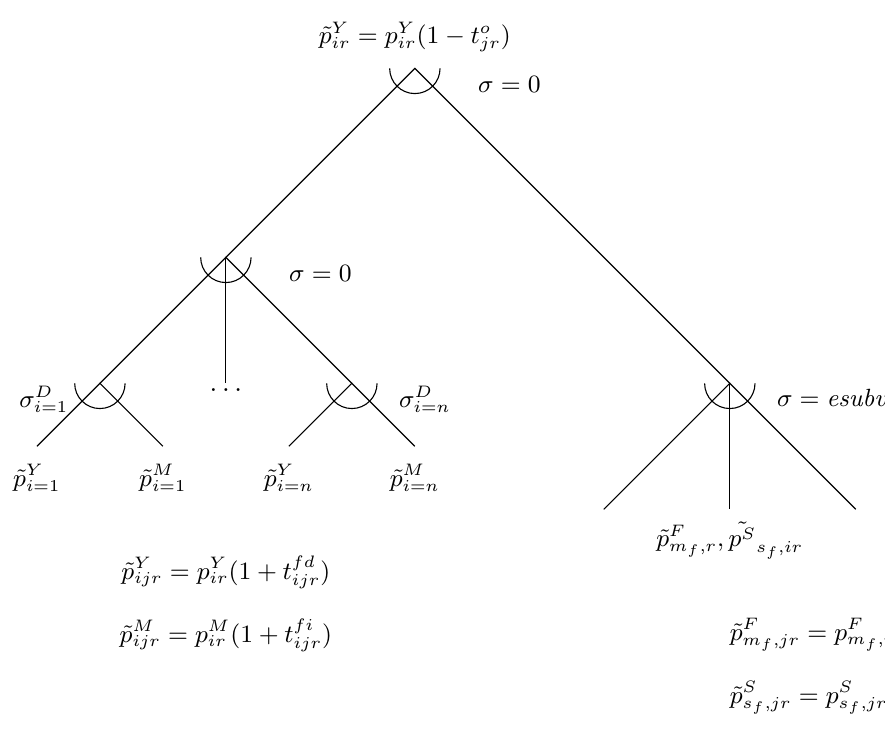
\begin{tikzpicture}[scale=0.8]
\node at (4,-1){\makebox(0,0)[c] {\small{$\tilde p^Y_{ijr} = p^Y_{ir} (1 + t^{fd}_{ijr})$}}};
\node at (4,-2){\makebox(0,0)[c]{\small{$\tilde p^M_{ijr} = p^M_{ir} (1 + t^{fi}_{ijr})$}}};
\node at (12,-2){\makebox(0,0)[l]{\small{$\tilde p^F_{m_f,jr} = p^F_{m_f,r} (1 + t^f_{m_f,jr})$}}};
\node at (12,-3){\makebox(0,0)[l]{\small{$\tilde p^S_{s_f,jr} = p^S_{s_f,jr} (1 + t^f_{s_f,jr})$}}};
%\node at (12,-4){\makebox(0,0)[l]{\small{$\sigma^D_i = \textit{esubd}_i$}}};
\node at (4,1.9){\makebox(0,0)[c]{$\ldots$}};
\node at (7,7.5){\makebox(0,0)[c]{\small{$\tilde p^Y_{ir} = p^Y_{ir} (1-t^o_{jr})$}}};
\node at (1,0.5){\makebox(0,0)[c]{\small{$\tilde p^Y_{i=1}$}}};
\node at (3,0.5){\makebox(0,0)[c]{\small{$\tilde p^M_{i=1}$}}};
\node at (5,0.5){\makebox(0,0)[c]{\small{$\tilde p^Y_{i=n}$}}};
\node at (7,0.5){\makebox(0,0)[c]{\small{$\tilde p^M_{i=n}$}}};
\node at (12,-0.5){\makebox(0,0)[c]{\small{$\tilde p^F_{m_f,r},\tilde{p^S}_{s_f,ir}$}}};
\node at (8.5,6.75){\makebox(0,0)[c]{\small{$\sigma=0$}}};
\node at (5.5,3.75){\makebox(0,0)[c]{\small{$\sigma=0$}}};
\node at (1.5,1.75){\makebox(0,0)[r]{\small{$\sigma^D_{i=1}$}}};
\node at (6.75,1.75){\makebox(0,0)[l]{\small{$\sigma^D_{i=n}$}}};
\node at (12.75,1.75){\makebox(0,0)[l]{\small{$\sigma=\textit{esubva}_i$}}};
\draw (2.4,2) arc (0:-180:0.4cm);
\draw (4.4,4) arc (0:-180:0.4cm);
\draw (6.4,2) arc (0:-180:0.4cm);
\draw (7.4,7) arc (0:-180:0.4cm);
\draw (12.4,2) arc (0:-180:0.4cm);
\draw (1,1)--(2,2)--(3,1);
\draw (5,1)--(6,2)--(7,1);
\draw (2,2)--(4,4)--(6,2);
\draw (4,4)--(4,2);
\draw (4,4)--(7,7)--(12,2);
\draw (10,0)--(12,2)--(14,0);
\draw (12,2)--(12,0);
\end{tikzpicture}
\end{filecontents*}

\begin{filecontents*}{figures/prodfunDX.tikz}
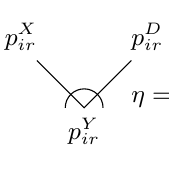
\begin{tikzpicture}[scale=0.6]
\draw (1,2)--(2,1)--(3,2);
\draw (2.4,1) arc (0:180:0.4cm);
\node at (3,1.25){\makebox(0,0)[l]{\small{$\eta=\textit{etrndx}_{i}$}}};
\node at (1,2.5){\makebox(0,0)[r]{\small{$p^X_{ir}$}}};
\node at (3,2.5){\makebox(0,0)[l]{\small{$p^D_{ir}$}}};
\node at (2,0.5){\makebox(0,0)[c]{\small{$p^Y_{ir}$}}};
\end{tikzpicture}
\end{filecontents*}

\begin{filecontents*}{figures/prodfunA.tikz}
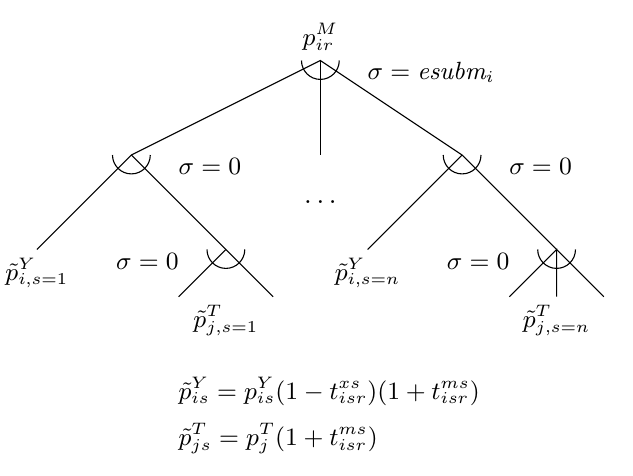
\begin{tikzpicture}[scale=0.6]
\node at (8,5.75){\makebox(0,0)[l]{\small{$\sigma=\textit{esubm}_i$}}};
\node at (4,3.75){\makebox(0,0)[l]{\small{$\sigma=0$}}};
\node at (11,3.75){\makebox(0,0)[l]{\small{$\sigma=0$}}};
\node at (4,1.75){\makebox(0,0)[r]{\small{$\sigma=0$}}};
\node at (11,1.75){\makebox(0,0)[r]{\small{$\sigma=0$}}};
\draw (1,2)--(3,4)--(7,6)--(10,4)--(12,2)--(13,1);
\draw (3,4)--(5,2);
\draw (4,1)--(5,2)--(6,1);
\draw (7,6)--(7,4);
\draw (8,2)--(10,4);
\draw (11,1)--(12,2)--(12,1);
\draw (3.4,4) arc (0:-180:0.4cm);
\draw (7.4,6) arc (0:-180:0.4cm);
\draw (5.4,2) arc (0:-180:0.4cm);
\draw (10.4,4) arc (0:-180:0.4cm);
\draw (12.4,2) arc (0:-180:0.4cm);
\node at (7,6.5){\makebox(0,0)[c]{\small{$p^M_{ir}$}}};
\node at (1,1.5){\makebox(0,0)[c]{\small{$\tilde{p}^Y_{i,s=1}$}}};
\node at (5,0.5){\makebox(0,0)[c]{\small{$\tilde{p}^T_{j,s=1}$}}};
\node at (8,1.5){\makebox(0,0)[c]{\small{$\tilde{p}^Y_{i,s=n}$}}};
\node at (12,0.5){\makebox(0,0)[c]{\small{$\tilde{p}^T_{j,s=n}$}}};
\node at (7,3){\makebox(0,0)[c]{$\ldots$}};
\node at (4,-1){\makebox(0,0)[l]{\small{$\tilde{p}^Y_{is} = p^Y_{is} (1 - t^{xs}_{isr})(1 + t^{ms}_{isr})$}}};
\node at (4,-2){\makebox(0,0)[l]{\small{$\tilde{p}^T_{js} = p^T_j (1 + t^{ms}_{isr})$}}};
\end{tikzpicture}
\end{filecontents*}


\begin{filecontents*}{figures/gtapflowchart.tikz}
\tikzset{%
  block/.style    = {draw, thick, rectangle, minimum height = 3em,
    minimum width = 3em},
  sum/.style      = {draw, circle, node distance = 2cm}, % Adder
  input/.style    = {coordinate}, % Input
  output/.style   = {coordinate} % Output
}
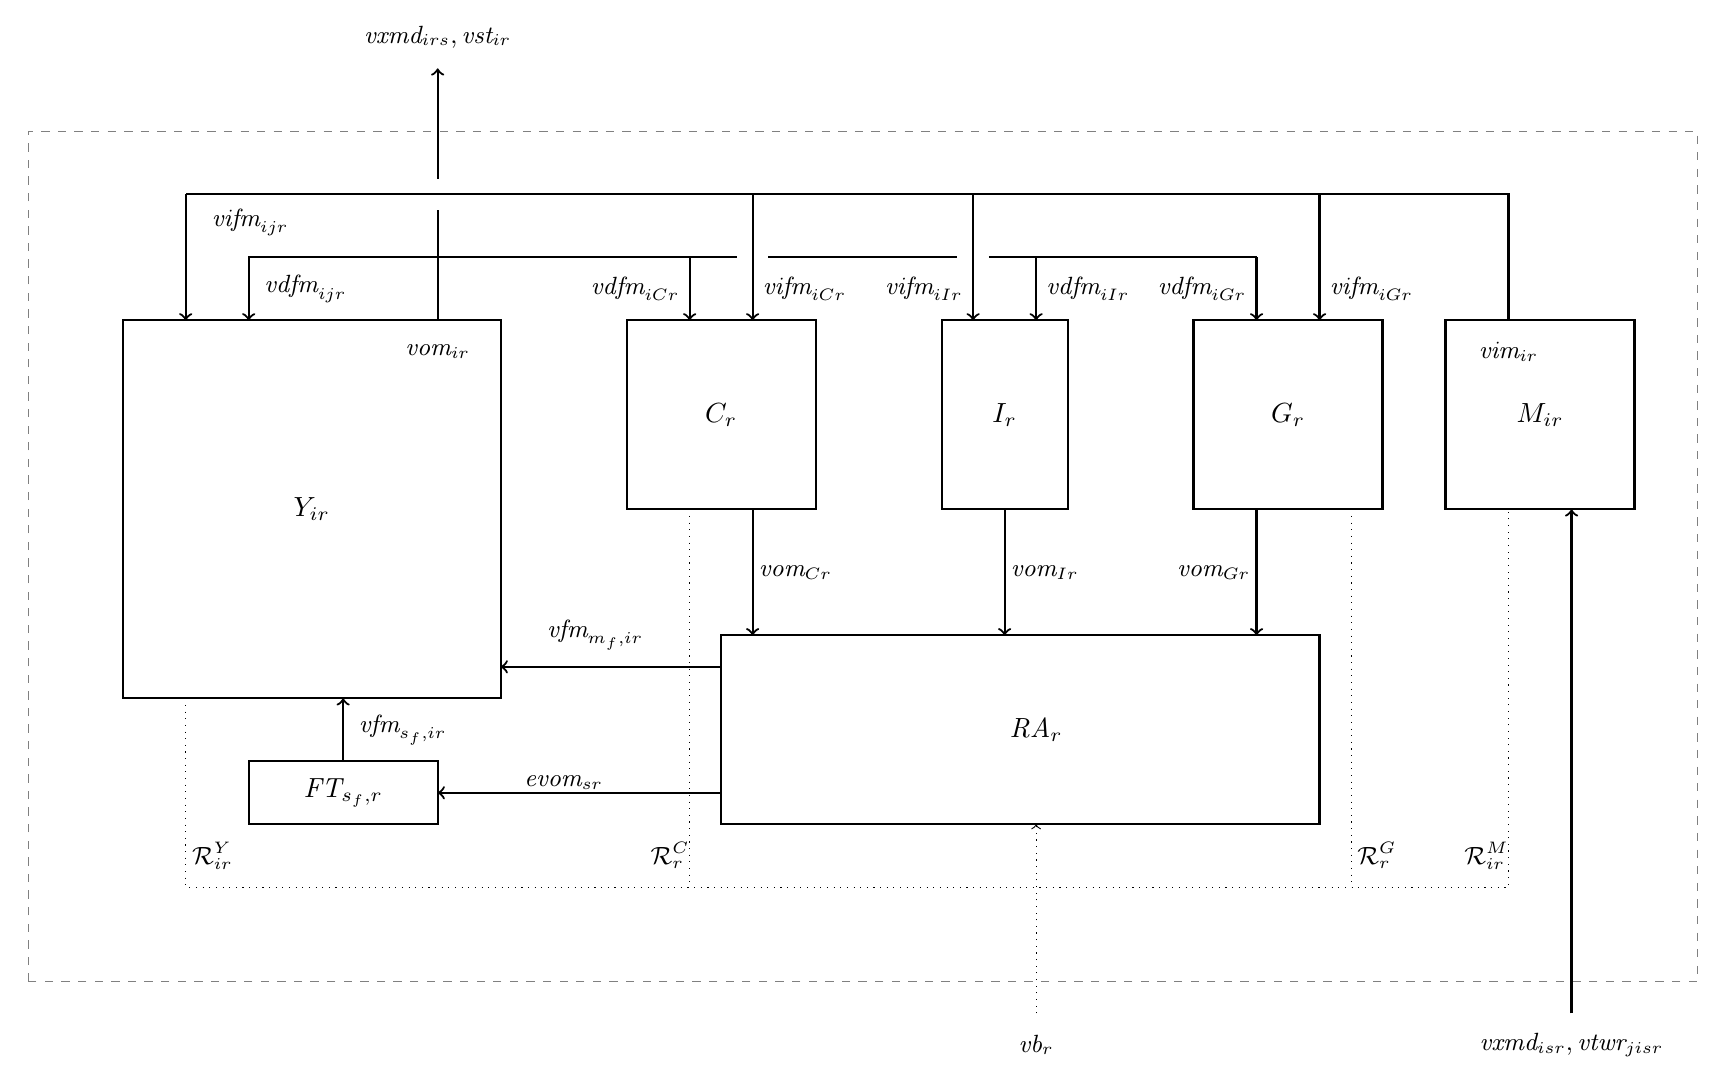
\begin{tikzpicture}[auto, thick, scale=0.8]
\draw[gray,thin,dashed] (-2.5,-0.5) rectangle (24,13);

\draw (-1,4)  rectangle (5,10);
\node at (2,7) {$Y_{ir}$};

\draw (1,2)   rectangle (4,3);
\node at (2.5,2.5) {$\textit{FT}_{s_{f},r}$};

\draw (8.5,2) rectangle (18,5);
\node at (13.5,3.5)  {$\textit{RA}_r$};

\draw (7,7) rectangle (10,10);
\node at (8.5,8.5) {$C_r$};

\draw (12,7) rectangle (14,10);
\node at (13,8.5) {$I_r$};

\draw (16,7) rectangle (19,10);
\node at (17.5,8.5) {$G_r$};

\draw (20,7) rectangle (23,10);
\node at (21.5,8.5) {$M_{ir}$};


\node [right] at (0.25,11.55) {\small{$\textit{vifm}_{ijr}$}};


\draw[thin,dotted] (0,4)--(0,1)--(21,1)--(21,7);  % Y to M (GOVT)
\node at (0.1,1.5) {\makebox(0,0)[l]{\small{$\mathcal{R}^Y_{ir}$}}};

\draw[thin,dotted] (8,7)--(8,1);              % C to GOVT
\node at (8,1.5) {\makebox(0,0)[r]{\small{$\mathcal{R}^C_r$}}};

%\dottedline{0.1}(13,7)(13,1)           % I to GOVT

\draw[->,thin,dotted] (13.5,-1)--(13.5,2);       % G to GOVT
\node at (13.5,-1.5){\makebox(0,0)[c]{\small{$\textit{vb}_r$}}};

\node at (18.6,1.5) {\makebox(0,0)[l]{\small{$\mathcal{R}^G_r$}}};
\node at (21,1.5) {\makebox(0,0)[r]{\small{$\mathcal{R}^M_{ir}$}}};

\draw[thin,dotted] (18.5,7)--(18.5,1);        % M to GOVT
%\draw[thin,dotted] (10.5,2)--(10.5,1);        % HH to GOVT

\draw (21,10)--(21,12)--(0,12);               % M to market
\node at (21,9.5){\makebox(0,0)[c]{\small{$\textit{vim}_{ir}$}}};
\draw (4,10)--(4,11)--(8.75,11);              % Y to market
\node at (4,9.5){\makebox(0,0)[c]{\small{$\textit{vom}_{ir}$}}};

\draw (4,11)--(4,11.75);             % Y to ROW
\draw (4,12.25)--(4,13.75);
\draw [->] (4,13.75)--(4,14);
\node at (4,14.5){\makebox(0,0)[c]{\small{$\textit{vxmd}_{irs},\textit{vst}_{ir}$}}};
\draw (4,11)--(1,11)--(1,10.25);              % Y to Y
\draw [->] (1,10.25)--(1,10);      % Y to Y
\node at (1.25,10.5) {\makebox(0,0)[l]{\small{$\textit{vdfm}_{ijr}$}}};

\draw  (9.25,11)--(12.25,11);            % Y to market
\draw  (12.75,11)--(17,11);            % Y to market

\draw  (22,-1)--(22,6.75);            % ROW to M
\draw [->] (22,6.75)--(22,7);
%\put(22,7.5){\makebox(0,0)[c]{\small{$p^Y_{is}, p^T_j$}}}

\node at (22,-1.5) {\makebox(0,0)[c]{\small{$\textit{vxmd}_{isr},\textit{vtwr}_{jisr}$}}};
\draw[->] (0,12)--(0,10);     % M to Y

\draw[->] (8,11)--(8,10);     % Y to C
\node [left]  at (8,10.5) {\small{$\textit{vdfm}_{iCr}$}};

\draw[->] (9,12)--(9,10);     % M to C
\node [right] at (9,10.5) {\small{$\textit{vifm}_{iCr}$}};

\draw[->] (12.5,12)--(12.5,10);   % M to I
\node [left] at (12.5,10.5) {\small{$\textit{vifm}_{iIr}$}};

\draw[->] (13.5,11)--(13.5,10);   % Y to I
\node [right] at (13.5,10.5) {\small{$\textit{vdfm}_{iIr}$}};

\node [left]  at (17,10.5) {\small{$\textit{vdfm}_{iGr}$}};
\node [right] at (18,10.5) {\small{$\textit{vifm}_{iGr}$}};
\draw[->] (17,11)--(17,10);   % Y to G
\draw[->] (18,12)--(18,10);   % M to G

\draw (9,7)--(9,5.25);          % C to HH
%\put(9,7.5){\makebox(0,0)[c]{\small{$p^C_{r}$}}}
\node  at (9.1,6){\makebox(0,0)[l]{\small{$\textit{vom}_{Cr}$}}};

\draw (13,7)--(13,5.25);        % I to HH
%\put(12,7.5){\makebox(0,0)[c]{\small{$p^Y_{\mbox{\textsc{cgd}},r}$}}}
\node at (13.1,6){\makebox(0,0)[l]{\small{$\textit{vom}_{Ir}$}}};
\draw (17,7)--(17,5.25);        % G to GOVT
%\put(17,7.5){\makebox(0,0)[c]{\small{$p^G_{r}$}}}

\draw (5.25,4.5)--(8.5,4.5);            % HH to Y
\draw[->] (5.25,4.5)--(5,4.5);     % HH to Y
\node at (6.5,5.0){\makebox(0,0)[c]{\small{$\textit{vfm}_{m_{f},ir}$}}};
%\put(4.75,3.5){\makebox(0,0)[r]{\small{$p^F_{fr},p^S_{fir}$}}}

\draw[<-] (4,2.5)--(8.5,2.5);     % HH to FT
\node[above] at (6,2.5) {\makebox(0,0)[c]{\small{$\textit{evom}_{sr}$}}};

\draw (2.5,3)--(2.5,3.75);              % FT to Y
\draw[->] (2.5,3.75)--(2.5,4);      % HH to FT
\node at (2.75,3.5){\makebox(0,0)[l]{\small{$\textit{vfm}_{s_{f},ir}$}}};

\draw[->] (9,5.25)--(9,5);       % C to HH
\draw[->] (13,5.25)--(13,5);      % I to HH

\draw[->] (17,5.25)--(17,5);      % G to GOVT
\node at (16.9,6){\makebox(0,0)[r]{\small{$\textit{vom}_{Gr}$}}};
\end{tikzpicture}
\end{filecontents*}

\begin{filecontents*}{figures/prodfunC.tikz}
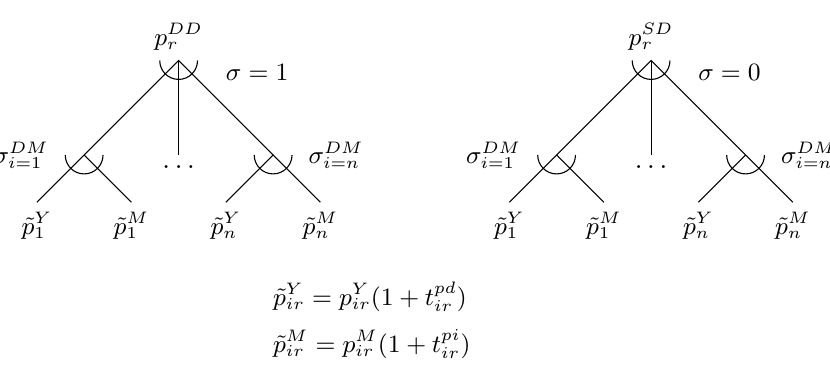
\begin{tikzpicture}[scale=0.6]
\draw(1,1)--(2,2)--(4,4)--(6,2)--(7,1);
\draw(2,2)--(3,1);
\draw(5,1)--(6,2);
\draw (4,2)--(4,4);
\node at (4,1.75){\makebox(0,0)[c]{$\ldots$}};
\draw (4.4,4) arc (0:-180:0.4cm);
\draw (2.4,2) arc (0:-180:0.4cm);
\draw (6.4,2) arc (0:-180:0.4cm);
\node at (5,3.75){\makebox(0,0)[l]{\small{$\sigma=1$}}};
\node at (1.25,2){\makebox(0,0)[r]{\small{$\sigma^{DM}_{i=1}$}}};
\node at (6.75,2){\makebox(0,0)[l]{\small{$\sigma^{DM}_{i=n}$}}};
\node at (1,0.5){\makebox(0,0)[c]{\small{$\tilde{p}^Y_{1}$}}};
\node at (3,0.5){\makebox(0,0)[c]{\small{$\tilde{p}^M_{1}$}}};
\node at (5,0.5){\makebox(0,0)[c]{\small{$\tilde{p}^Y_{n}$}}};
\node at (7,0.5){\makebox(0,0)[c]{\small{$\tilde{p}^M_{n}$}}};
\node at (4,4.5){\makebox(0,0)[c]{\small{$p^{DD}_r$}}};
\node at (6,-1){\makebox(0,0)[l]{\small{$\tilde{p}^Y_{ir} = p^Y_{ir} (1 + t^{pd}_{ir})$}}};
\node at (6,-2){\makebox(0,0)[l]{\small{$\tilde{p}^M_{ir} = p^M_{ir} (1 + t^{pi}_{ir})$}}};
\draw(11,1)--(12,2)--(14,4)--(16,2)--(17,1);
\draw(12,2)--(13,1);
\draw(15,1)--(16,2);
\draw (14,2)--(14,4);
\node at (14,1.75){\makebox(0,0)[c]{$\ldots$}};
\draw (14.4,4) arc (0:-180:0.4cm);
\draw (12.4,2) arc (0:-180:0.4cm);
\draw (16.4,2) arc (0:-180:0.4cm);
\node at (15,3.75){\makebox(0,0)[l]{\small{$\sigma=0$}}};
\node at (11.25,2){\makebox(0,0)[r]{\small{$\sigma^{DM}_{i=1}$}}};
\node at (16.75,2){\makebox(0,0)[l]{\small{$\sigma^{DM}_{i=n}$}}};
\node at (11,0.5){\makebox(0,0)[c]{\small{$\tilde{p}^Y_{1}$}}};
\node at (13,0.5){\makebox(0,0)[c]{\small{$\tilde{p}^M_{1}$}}};
\node at (15,0.5){\makebox(0,0)[c]{\small{$\tilde{p}^Y_{n}$}}};
\node at (17,0.5){\makebox(0,0)[c]{\small{$\tilde{p}^M_{n}$}}};
\node at (14,4.5){\makebox(0,0)[c]{\small{$p^{SD}_r$}}};
\end{tikzpicture}
\end{filecontents*}

\begin{filecontents*}{figures/prodfunFT.tikz}
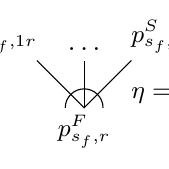
\begin{tikzpicture}[scale=0.6]
\draw (1,2)--(2,1)--(3,2);
\draw (2,1)--(2,2);
\draw (2.4,1) arc (0:180:0.4cm);
\node at (2,2.25){\makebox(0,0)[c]{$\ldots$}};
\node at (3,1.25){\makebox(0,0)[l]{\small{$\eta=\textit{etrae}_{s_{f}}$}}};
\node at (1,2.5){\makebox(0,0)[r]{\small{$p^S_{s_{f},1r}$}}};
\node at (3,2.5){\makebox(0,0)[l]{\small{$p^S_{s_{f},nr}$}}};
\node at (2,0.5){\makebox(0,0)[c]{\small{$p^F_{s_{f},r}$}}};
\end{tikzpicture}
\end{filecontents*}

\begin{filecontents*}{figures/prodfunYT.tikz}
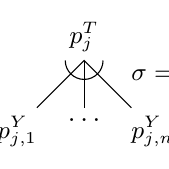
\begin{tikzpicture}[scale=0.6]
\draw(1,1)--(2,2)--(3,1);
\draw(2,1)--(2,2);
\draw (2.4,2) arc (0:-180:0.4cm);
\node at (2,0.75){\makebox(0,0)[c]{$\ldots$}};
\node at (3,1.75){\makebox(0,0)[l]{\small{$\sigma=1$}}};
\node at (1,0.5){\makebox(0,0)[r]{\small{$p^Y_{j,1}$}}};
\node at (3,0.5){\makebox(0,0)[l]{\small{$p^Y_{j,n}$}}};
\node at (2,2.5){\makebox(0,0)[c]{\small{$p^T_j$}}};
\end{tikzpicture}
\end{filecontents*}

\begin{filecontents*}{figures/prodfunG.tikz}
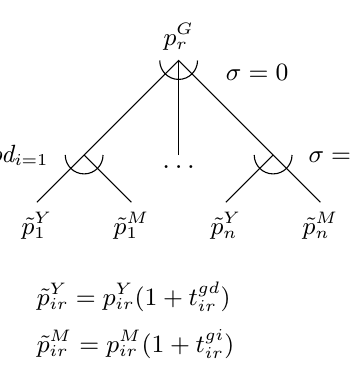
\begin{tikzpicture}[scale=0.6]
\draw(1,1)--(2,2)--(4,4)--(6,2)--(7,1);
\draw(2,2)--(3,1);
\draw(5,1)--(6,2);
\draw (4,2)--(4,4);
\node at (4,1.75){\makebox(0,0)[c]{$\ldots$}};
\draw (4.4,4) arc (0:-180:0.4cm);
\draw (2.4,2) arc (0:-180:0.4cm);
\draw (6.4,2) arc (0:-180:0.4cm);
\node at (5,3.75){\makebox(0,0)[l]{\small{$\sigma=0$}}};
\node at (1.25,2){\makebox(0,0)[r]{\small{$\sigma=\textit{esubd}_{i=1}$}}};
\node at (6.75,2){\makebox(0,0)[l]{\small{$\sigma=\textit{esubd}_{i=n}$}}};
\node at (1,0.5){\makebox(0,0)[c]{\small{$\tilde{p}^Y_{1}$}}};
\node at (3,0.5){\makebox(0,0)[c]{\small{$\tilde{p}^M_{1}$}}};
\node at (5,0.5){\makebox(0,0)[c]{\small{$\tilde{p}^Y_{n}$}}};
\node at (7,0.5){\makebox(0,0)[c]{\small{$\tilde{p}^M_{n}$}}};
\node at (4,4.5){\makebox(0,0)[c]{\small{$p^G_r$}}};
\node at (1,-1){\makebox(0,0)[l]{\small{$\tilde{p}^Y_{ir} = p^Y_{ir}
(1 + t^{gd}_{ir})$}}};
\node at (1,-2){\makebox(0,0)[l]{\small{$\tilde{p}^M_{ir} = p^M_{ir}
(1 + t^{gi}_{ir})$}}};
\end{tikzpicture}
\end{filecontents*}

\begin{filecontents*}{figures/figure9a.tikz}
\begin{tikzpicture}
 \pgfplotsset{filter discard warning=false}
\begin{axis}[
%  legend cell align=left,
%  height=0.4\textheight,
  xlabel shift = 0.05in,
  ylabel shift = -0.05in,
  xlabel={Quantity ($q$)},
  ylabel={Price ($p$)},
  axis line style={->},
  axis x line* = bottom,
  axis y line = left,
  grid = major,
  grid style={dashed, gray!30},
  xmin = 0,
  xmax = 3,
  ymin = 0.8,
  ymax = 1.4]
\addplot[color=red, thick, solid] table [y=p, x=q]{figures/figure9.data};
\addplot[color=blue, thick,  dashed] table [y=pref, x=q]{figures/figure9.data};
\node[circle,label={135:$b$},fill=black,scale=0.3] at (axis cs:1,1)     {};
\node[circle,label={ 45:$a$},fill=black,scale=0.3] at (axis cs:1,1.2)   {};
\node[circle,label={-135:$c$},fill=black,scale=0.3] at (axis cs:2.48832,1) {};
\end{axis}
\end{tikzpicture}
\end{filecontents*}{figures/figure9a.tikz}

\begin{filecontents*}{figures/figure9b.tikz}
\begin{tikzpicture}
\pgfplotsset{filter discard warning=false}
\begin{axis}[
%  legend cell align=left,
%  height=0.4\textheight,
  xlabel shift = 0.05in,
  ylabel shift = -0.05in,
  xlabel={Quantity ($q$)},
  ylabel={Price ($p$)},
  axis line style={->},
  axis x line* = bottom,
  axis y line = left,
  grid = major,
  grid style={dashed, gray!30},
  xmin = 0,
  xmax = 3,
  ymin = 0.8,
  ymax = 1.4]
\addplot[color=red,  thick, solid] table [y=p, x=d]{figures/figure9.data};
\addplot[color=blue, thick, dashed] table [y=p, x=s]{figures/figure9.data};
\addplot[color=red,  thin,  solid] table [y=p, x=q]{figures/figure9.data};
\addplot[color=blue, thin,  dashed] table [y=pref, x=q]{figures/figure9.data};
\draw [color=black, thin, dashed] (axis cs:2.48832,0.8) -- (axis cs:2.48832,1.18) -- (axis cs:0,1.18);
\node[circle,label={135:$b$},fill=black,scale=0.3] at (axis cs:1,1)     {};
\node[circle,label={ 45:$a$},fill=black,scale=0.3] at (axis cs:1,1.2)   {};
\node[circle,label={-135:$c$},fill=black,scale=0.3] at (axis cs:2.48832,1) {};
\node[circle,label={-45:$d$},fill=black,scale=0.3] at (axis cs:2.48832,1.18) {};
\end{axis}
\end{tikzpicture}
\end{filecontents*}{figures/figure9b.tikz}

%	The data presented here has been copied from ExportElasticity.xlsx
%	in the LaTeX/figures directory:

\begin{filecontents}{figures/figure9.data}
p	q		pref	d		s
nan	0		1.0	nan		nan
1.3	0.670176922	1.0	0.01827657	4.29554847
1.29	0.696558632	1.0	0.026889132	4.115165249
1.28	0.724196434	1.0	0.039679283	3.941040905
1.27	0.753160657	1.0	0.058732198	3.773004634
1.26	0.783526166	1.0	0.087203727	3.610889011
1.25	0.815372698	1.0	0.129885794	3.454529941
1.24	0.848785212	1.0	0.194078776	3.303766628
1.23	0.883854288	1.0	0.290942208	3.158441529
1.22	0.92067654	1.0	0.437593406	3.018400312
1.21	0.959355078	1.0	0.660379809	2.883491822
1.2	1		1.0	1		2.753568034
1.19	1.042728931	1.0	1.519547333	2.62848402
1.18	1.087667605	1.0	2.317191555	2.508097903
1.17	1.134950503	1.0	3.546248908	2.39227082
1.16	1.184721539	1.0	5.447068553	2.280866886
1.15	1.237134814	1.0	8.397891991	2.173753149
1.14	1.292355435	1.0	nan		2.070799555
1.13	1.350560404	1.0	nan		1.971878908
1.12	1.411939594	1.0	nan		1.876866831
1.11	1.476696809	1.0	nan		1.785641729
1.1	1.545050947	1.0	nan		1.698084751
1.09	1.617237267	1.0	nan		1.614079749
1.08	1.693508781	1.0	nan		1.533513242
1.07	1.77413777	1.0	nan		1.456274381
1.06	1.859417457	1.0	nan		1.382254907
1.05	1.949663831	1.0	nan		1.311349117
1.04	2.045217658	1.0	nan		1.243453825
1.03	2.14644669	1.0	nan		1.178468328
1.02	2.253748089	1.0	nan		1.116294364
1.01	2.3675511	1.0	nan		1.056836081
1	2.48832		1.0	nan		1
0.99	2.616557345	1.0	nan		0.945694974
0.98	2.752807557	1.0	nan		0.893832159
0.97	2.897660889	1.0	nan		0.844324973
0.96	3.051757813	1.0	nan		0.797089063
0.95	3.215793876	1.0	nan		0.75204227
0.94	3.390525088	1.0	nan		0.709104592
0.93	3.576773897	1.0	nan		0.668198151
0.92	3.775435834	1.0	nan		0.629247158
0.91	3.987486894	1.0	nan		0.592177878
0.9	4.21399177	1.0	nan		0.556918595
0.89	4.456113017	1.0	nan		0.523399581
0.88	4.715121297	1.0	nan		0.491553056
0.87	4.992406813	1.0	nan		0.461313164
0.86	5.289492114	1.0	nan		0.43261593
0.85	5.608046444	1.0	nan		0.405399231
0.84	5.949901827	1.0	nan		0.379602765
\end{filecontents}


\begin{document}
\title{Documentation of \GTAPINGAMS}
\author{}
\date{}
%
\maketitle

\begin{abstract} % Environment defined for JGEA style.

This paper describes the implementation in the General Algebraic
Modeling Language (\GAMS) of an economic equilibrium model based on
the Global Trade Analysis Project (\GTAP) dataset. We call this model
and the ancillary programming tools \GTAPINGAMS.  Relative to previous
installments of \GTAPINGAMS, an innovation in this model is that it
can easily switch between global multiregional (\GMR) and small open
economy (\SOE) closures. We also include the possibility to compare
results for alternative representations of final demand, based on
Cobb-Douglas, linear expenditure system and constant difference in
elasticities demand systems. In this paper we outline the model
structure, document the associated equilibrium conditions and describe
computer programs which calibrate the model to the desired regional
and sectoral aggregation from the \GTAP12 dataset.

\end{abstract}

\section{Data, Technology and Preferences}\label{model}

This section introduces the structure of core \GMR and \SOE models
included in the \GTAPINGAMS distribution. Both models are static, and
track the production and distribution of goods in the global economy.
In the \GTAP 12 Data Base the world is divided into 163 regions
(typically representing individual countries) and 65 commodities (or
goods), but computational constraints tend to limit the number of
regions and goods which can be included in a single
model. Datasets are easily aggregated which can be useful for
both empirical applications focusing on a subset of regions and for
debugging steps at the model formulation stage.

In each region, final demand structure is composed of public and
private expenditure across goods. Decisions about the allocation of
resources are decentralized, and the representation of behavior by
consumers and firms in the model follows the canonical microeconomic
optimization framework: (i) consumers maximize welfare subject to a
budget constraint with fixed levels of investment and public
expenditure; (ii) producers combine intermediate inputs, and primary
factors (several categories of labor, land, resources and physical
capital) at least cost for given technology.\footnote{Details about
  \GTAP sectors and primary factors are provided in Appendix
  \ref{sectors}. Readers of this paper who are interested in using
  \GTAPINGAMS as a research tool are encouraged to refer to Appendix
  \ref{installation} for installation instructions. The computer
  programs described have been tested using data files from the \GTAP
  12 GDX package, contained in \texttt{GDX12a\_AY16994.zip}. A license
  for these data files must be purchased separately by the users. In
  addition, a licensed installation of \GAMS (version 24.7.3 or
  higher) is required. }

While \GMR and \SOE models are based on the same data and employ the
same representation of production technology and consumer preferences,
they of course differ in their representation of trade. The \GMR model
is based on a standard Armington representation of bilateral trade
flows. An implication is that production and consumption decisions in
a given country (or group of countries) will affect world prices, and
the magnitude of this effect will mainly depend on the elasticity
estimates (a measure of country-level market-power). By contrast, the
\SOE model considers the case in which production and consumption
decision in a region country (or group of country) do not affect world
prices. This is modeled by treating supply and demand by the ``rest of
the world'' (\textsc{row}, i.e. countries that are not considered
relevant for the \SOE analysis) as perfectly elastic.  Corner
solutions are avoided through the assumption that output destined for
the domestic and export markets are differentiated products
\citep[see][]{DeMeloRobinson1989}.\footnote{In the present
implementation, international closure between the region of interest
and the \textsc{row} is achieved by fixing the value of the current
account at its benchmark level, and permitting the real exchange rate
to clear the market. Other assumptions are of course possible and are
left for future research. } Therefore, from the perspective of a given
region, the impact of policy evaluated in \GMR and \SOE models will
differ through their impact on the terms of trade.

In the following, we start by describing the basic notation, and then
present the structure of the data together with benchmark accounting
identities. We then present a ``primal'' description of agents'
optimization problems (i.e. specified in terms of quantity variables),
which leads to the equilibrium conditions presented in the subsequent
section.

\subsection{Notation}

The notation used in the model is summarized in the Tables \ref{sets}
- \ref{prices}. Table \ref{sets} defines the various dimensions which
characterize an instance of the model, including the set of
sectors/commodities ($i,j$), the set of regions ($r,s)$, the set of
factors of production ($f$). Set $g$ combines the production sectors
$i$ and private and public consumption demand (indices \texttt{"C"}
and \texttt{"G"}) and investment demand (index \texttt{"I"}). It
allows for a much tighter formulation of the model as they can all be
conceived of ``goods'' produced in similar fashion. To simplify the
exposition of the model, however, we describe private consumption,
public consumption and investment demand as stand alone components.

\renewcommand{\arraystretch}{1}
\renewcommand{\tabcolsep}{1mm}
\begin{table}[t!]
\begin{center}
\caption{Definitions of set indices.} \label{sets}
\small
\begin{tabular}{lp{4in}}
\toprule
Set &Definition  \\
\addlinespace
\midrule
\addlinespace
$i,j$ & Sectors, an aggregation of the 65 sectors in the \GTAP 12
Data Base \\
$g$ & Production sectors $i$, plus private consumption \texttt{"C"},
public demand \texttt{"G"} and investment \texttt{"I"} \\
$r,s$ & Regions, an aggregation of the 163 regions in the
\GTAP 12 Data Base\\
$f$ & Factors of production (consisting of
\textit{mobile factors}, $f \in m_f$, skilled labor (i. officials,
mangers and legislators (ISCO-88 Major Groups 1-2), ii. technicians
and associated professionals, iii.
clerks, and iv. service and market sales workers), unskilled labor,
capital, and \textit{sector-specific}, $f \in s_f$, agricultural land
and other resources)\\ \addlinespace \bottomrule
\end{tabular}
\end{center}
\vspace{0.4in}
\end{table}

Table \ref{activities} defines the primal variables (activity levels)
which characterize an equilibrium. The model determines values of all
the variables except international capital flows, a parameter which
would be determined endogenously in an intertemporal model. Table
\ref{activities} also displays the concordance between the variables
and their \GAMS equivalents.

\renewcommand{\arraystretch}{1}
\renewcommand{\tabcolsep}{1mm}
\begin{table}[t!]
\begin{center}
\caption{Definitions of activity levels (quantity variables).} \label{activities}
\small
\begin{tabular}{lllr}
\toprule
Variable &Definition  & GAMS variable & Benchmark (\GTAP) value \\
\addlinespace
\midrule
\addlinespace
$Y_{ir}$&       Production & \texttt{Y(i,r)} &\texttt{vom(i,r)}\\
\\
$C_{r}$&        Discretionary consumption & \texttt{Y("c",r)} &\texttt{vom("c",r)}\\
\\
$G_{r}$&        Aggregate public & \texttt{Y("g",r)}&\texttt{vom("g",r)} \\
\\
$I_{r}$&        Aggregate investment & \texttt{Y("i",r)}&\texttt{vom("i",r)} \\
\\
$M_{ir}$&       Aggregate imports & \texttt{M(i,r)}&\texttt{vim(i,r)}\\
\\
$X_{ir}$&       Trade flows with rest of world regions &
\texttt{X(i,r)}&\texttt{vem(i,r)}\\
\\
$\textit{FT}_{fr}$&      Factor transformation &
\texttt{FT(f,r)}&\texttt{evom(f,r)}\\
\\
$\textit{YT}_j$  &       International transport services & \texttt{YT(j)}&\texttt{vtw(j)}\\
\addlinespace
\bottomrule
\end{tabular}
\end{center}
\vspace{0.4in}
\end{table}

Table \ref{prices} defines the relative price variables for goods and
factors in the model. As is the case in any Shoven-Whalley \CGE model,
the equilibrium conditions determine \textit{relative} rather than
\textit{nominal} prices.

\renewcommand{\arraystretch}{1}
\renewcommand{\tabcolsep}{1mm}
\begin{table}[t!]
\begin{center}
\caption{Definitions of price variables.} \label{prices}
\small
\begin{tabular}{lp{3in}r}
\toprule
Variable &Definition & GAMS variable\\
\addlinespace
\midrule
\addlinespace
$p^C_{r}$      &       Final demand price index for the Cobb-Douglas
demand system &\texttt{P("C",r)}\\
\\
$p^G_{r}$      &       Public provision price index  &\texttt{P("G",r)}\\
\\
$p^I_{r}$      &       Investment price index &\texttt{P("I",r)}\\
\\
$p^Y_{ir}$     &       Supply price, gross of indirect producer
taxes (when $\eta^{DX}_{i} < \infty$, the supply price is
replaced by and export price, $p^X_{ir}$ and domestic supply price,
$p^D_{ir}$) &\texttt{P(i,r)}\\
\\
$p^M_{ir}$     &       Import price, gross of export
taxes and tariffs.&\texttt{PM(i,r)}\\
\\
$p^E_{ir}$     &       Export price from endogenous or exogenous
regions.&\texttt{PE(i,r)}\\
\\
$p^T_j$         &       Marginal cost of transport services
&\texttt{PT(j)}\\
\\
$p^F_{f,r}$     &       Price of mobile primary factors ($m_f$
include labor, land and resources) &\texttt{PF(f,r)}\\
\\
$p^S_{s_f,ir}$     &       Price of sector-specific primary
factors&\texttt{PS(sf,i,j)}\\
\addlinespace
\bottomrule
\end{tabular}
\end{center}
\vspace{0.4in}
\end{table}

While the core \GTAPINGAMS model is base on Cobb-Douglas final demand,
the canonical models incorporate logic for two additional demand
systems: the \LES and the \CDE demand system. In particular, the \LES
representation distinguishes between subsistence demand and
discretionary demand, and we define the additional variables in Table
\ref{dsysprices}. Similarly, we define an Armington composite price
index for products entering \CDE final demand.  (Details of these
demand systems are provided in Appendices \ref{CDE} and \ref{LES}.)

\begin{table}[t!]
\begin{center}
\caption{Additional variables for \LES and \CDE demand systems.} \label{dsysprices}
\small
\begin{tabular}{lp{3in}r}
\toprule
Variable &Definition & GAMS variable\\
\addlinespace
\midrule
\addlinespace
$SD_{r}$&       Subsistence demand & \texttt{Y("sd",r)} \\
\\
$DD_{r}$&       Discretionary demand & \texttt{Y("dd",r)} \\
\\
$p^{DD}_{r}$   &       Discretionary demand price index &\texttt{P("dd",r)}\\
\\
$p^{SD}_{r}$   &       Subsistence demand price index &\texttt{P("sd",r)}\\
\\
$p^A_{iCr}$     &      Armington composite price representing the
market price of goods entering \CDE demand.&\texttt{PA(i,r)}\\
\addlinespace
\bottomrule
\end{tabular}
\end{center}
\vspace{0.4in}
\end{table}

Finally, Table \ref{taxes} reports the definition of tax and subsidy
rates applied in the model, both in terms of the notation employed to
describe the model and that used in the \GAMS code. Note that revenues
from taxes and subsidy expenditures do not appear as explicit
variables in the \GTAP Data Base and are defined on the basis of
expenditures and tax rates. We come back to this below.

\renewcommand{\arraystretch}{1}
\renewcommand{\tabcolsep}{1mm}
\begin{table}[t!]
\begin{center}
\caption{Tax and subsidy rates (net basis unless noted).} \label{taxes}
\small
\begin{tabular}{lp{6cm}lr}
\toprule
Parameter & Definition &  & \GAMS Parameter \\
\addlinespace
\midrule
\addlinespace
$t^o_{ir}$ & Output taxes (gross basis)& & \texttt{rto(i,r)}    \\
\\
$t^{f}_{fir}$   &Factor taxes &  & \texttt{rtf(f,i,r)}   \\
\\
$t^{fd}_{ijr}$ & Intermediate input taxes &Domestic&\texttt{rtfd(i,j,r)}      \\
$t^{fi}_{ijr}$ &                          &Imported& \texttt{rtfi(i,j,r)}      \\
\\
$t^{pd}_{ir}$ & Consumption taxes  & Domestic& \texttt{rtfd(i,"C",r)}     \\
$t^{pi}_{ir}$ &                 &Imported& \texttt{rtfi(i,"C",r)} \\
\\
$t^{gd}_{ir}$ & Public demand taxes &Domestic & \texttt{rtfd(i,"G",r)}   \\
$t^{gi}_{ir}$&                 &Imported & \texttt{rtfi(i,"G",r)} \\
\\
$t^{gd}_{ir}$ & Investment demand taxes &Domestic & \texttt{rtfd(i,"I",r)}   \\
$t^{gi}_{ir}$&                 &Imported& \texttt{rtfi(i,"I",r)} \\
\\
$t^{xs}_{isr}$  &Export subsidies&  & \texttt{rtxs(i,s,r)}   \\
\\
$t^{ms}_{isr}$  &Import tariffs& & \texttt{rtms(i,s,r)}\\
\addlinespace
\bottomrule
\end{tabular}
\end{center}
\vspace{0.4in}
\end{table}

\subsection[Accounting identities]{Benchmark data structure and accounting identities}

The economic structure underlying the \GTAP dataset and model is
illustrated in Figure \ref{fig:region}. Symbols in this flow chart
correspond to variables in the economic model (see Table
\ref{activities}): $Y_{ir}$ is the production of good $i$ in region
$r$, $C_r$, $I_r$ and $G_r$ portray private consumption, investment
and public demand, respectively, $M_{ir}$ portrays the import of good
$i$ into region $r$, $\textit{RA}_r$ stand for representative
consumers, and $FT_{s_{f}r}$ is the activity through which the set of
sector-specific factors of production ($s_f$) are allocated to
individual sectors. Further, solid lines represent commodity and
factor market flows, while dotted lines indicate tax revenues and
transfers.

\begin{sidewaysfigure}
\begin{center}
\includegraphics{figures/gtapflowchart.tikz}
\caption{Regional economic structure.} \label{fig:region}
\end{center}
\end{sidewaysfigure}

Domestic and imported goods markets are represented by horizontal
lines at the top of the figure. Domestic production
($\textit{vom}_{ir}$) is distributed to exports
($\textit{vxmd}_{irs}$), international transportation services
($\textit{vst}_{ir}$), intermediate demand ($\textit{vdfm}_{ijr}$),
household consumption ($\textit{vdfm}_{iCr}$), investment
($\textit{vdfm}_{iIr}$), and government consumption
($\textit{vdfm}_{iGr}$).\footnote{Recall that in the \GAMS
implementation of the model the index \texttt{"g"} includes all
sectors represented in the model plus private consumption
\texttt{"C"}, public demand \texttt{"G"} and investment \texttt{"I"}.
(See Table \ref{sets}.) For the LES demand representation, it also
includes price indices for discretionary demand \texttt{"dd"} and
subsistence demand \texttt{"sd"}. } The accounting identity in the
\GTAP 12 dataset is thus:
$$\textit{vom}_{ir} = \sum_s \textit{vxmd}_{irs} + \textit{vst}_{ir}
+ \sum_j \textit{vdfm}_{ijr} + \textit{vdfm}_{iCr} +
\textit{vdfm}_{iIr} + \textit{vdfm}_{iGr}\,,$$ where $j$ indexes all
goods. Similarly, imported goods (with aggregate value
$\textit{vim}_{ir}$) enter intermediate demand
($\textit{vifm}_{ijr}$), private consumption ($\textit{vifm}_{iCr} +
\textit{vifm}_{i\textit{SD}r}$)
and public consumption ($\textit{vifm}_{iGr}$). The accounting
identity for these flows is thus:
$$\textit{vim}_{ir} = \sum_j \textit{vifm}_{ijr} +
\textit{vifm}_{iCr} + \textit{vifm}_{i\textit{SD}r} + \textit{vifm}_{iGr}\,.$$

Inputs to production of good $i$ ($Y_{ir}$) include intermediate
inputs (domestic $\textit{vdfm}_{ijr}$ and imported
$\textit{vifm}_{ijr}$), mobile factors of production
($\textit{vfm}_{m_{f},ir}$, where $m_{f}$ is a subset of the set $f$
designating all factors of production), and sector-specific factors of
production ($\textit{vfm}_{s_{f},ir}, s_f \subset f$). Factor market
equilibrium is given by an identity relating the value of factor
payments to factor income:
$$\sum_i \textit{vfm}_{fir} = \textit{evom}_{fr}\,,$$ and factor
earnings accrue to households.

International market clearance conditions require that region $r$
exports of good $i$ ($\textit{vxmd}_{ir}$ at the top of the figure)
equal the imports of the same good from the same region summed across
all trading partners ($\textit{vxmd}_{isr}$ at the bottom of the
figure): $$\textit{vxm}_{ir} = \sum_s \textit{vxmd}_{irs}\,,$$ where
$s$, an alias for $r$, indexes regions. Likewise, market clearance
conditions apply for international transportation services. The
supply-demand balance in the market for transportation service $j$
requires that the sum across all regions of service exports
($\textit{vst}_{ir}$, at the top of the figure) equals the sum across
all bilateral trade flows of service inputs ($\textit{vtwr}_{jisr}$ at
the bottom of the figure):
$$\sum_r \textit{vst}_{jr} = \sum_{isr} \textit{vtwr}_{jisr}$$

Turning to tax revenues and transfers, shown as dotted lines in figure
\ref{fig:region}, flows labeled with $\mathcal{R}$ correspond to tax
revenues. For each country, tax flows consist of indirect taxes on
production/exports of each good ($\mathcal{R}^Y_{ir}$), on consumption
($\mathcal{R}^C_r$), on public demand ($\mathcal{R}^G_r$) and on
imports ($\mathcal{R}^M_{ir}$). The regional budget constraint thus
relates tax payments ($\mathcal{R}^Y_{ir}, \mathcal{R}^C_r,
\mathcal{R}^G_r, \mathcal{R}^M_{ir}$), factor income
($\textit{evom}_{fr}$), and the current account deficit (i.e., net
transfers from abroad, $\textit{vb}_r$) to total private consumption
expenditure $\textit{vom}_{Cr}$, total public consumption expenditure
$\textit{vom}_{Gr}$, and total investment $\textit{vom}_{Ir}$,
yielding:
$$\textit{vom}_{Cr} + \textit{vom}_{Gr} + \textit{vom}_{Ir} = \sum_f
\textit{evom}_{fr} + \sum_i \mathcal{R}^Y_{ir} + \mathcal{R}^C_r +
\mathcal{R}^G_r + \sum_i \mathcal{R}^M_{ir} + \textit{vb}_r\,. $$

To this point we have outlined two types of consistency conditions
which are part of any \GTAP Data Base: market clearance (supply = demand
for all goods and factors), and income balance (net income = net
expenditure). A third set of identities involve net operating profits
by all sectors in the economy. In the core \GTAP model ``production''
takes place under conditions of perfect competition with constant
returns to scale, hence there are no excess profits, and the cost of
inputs must equal the value of outputs. This condition applies for
each production sector:

\begin{itemize}
\item[$Y_{ir}$:] $\sum_f \textit{vfm}_{fir} + \sum_j
\left(\textit{vdfm}_{ijr} + \textit{vifm}_{ijr} \right) +
\mathcal{R}^Y_{ir} = \textit{vom}_{ir}\,,$
\item[$C_{r}$:] $\sum_i \left(\textit{vdfm}_{iCr} +
\textit{vifm}_{iCr} \right) + \mathcal{R}^C_{ir} = \textit{vom}_{Cr}\,,$
\item[$I_{r}$:] $\sum_i \textit{vdfm}_{iIr} = \textit{vom}_{Ir}$
\item[$G_{r}$:] $\sum_i \left(\textit{vdfm}_{iGr} +
\textit{vifm}_{iGr} \right) + \mathcal{R}^G_{ir} =
\textit{vom}_{Gr}\,,$
\item[$M_{ir}$:] $\sum_s \left(\textit{vxmd}_{isr} + \sum_j
\textit{vtwr}_{jisr} \right) + \mathcal{R}^M_{ir} = \textit{vim}_{ir}$
\item[$FT_{fr}$:] $\textit{evom}_{fr} = \sum_i \textit{vfm}_{fir}$
\end{itemize}

\subsection[Optimization problems]{Decentralized optimization problems}

The benchmark identities presented in the previous section indicate
the market clearance, zero profit and income balance conditions which
define the \GTAP model. The displayed equations do not, however,
characterize the behavior of agents in the model. In a competitive
equilibrium setting, the standard assumption of optimizing atomistic
agents applies for both producers and consumers. This section lays out
the optimization problem of each component in the model, and thereby
provides the structure of production technology (production functions)
and preferences (characterizing final demand), as well as the
representation of trade. We also highlight where conceptual
differences between \GMR and \SOE models intervene.

Note that in order to simplify notation, we denote decision variables
corresponding to the benchmark data structures with the initial ``v''
replaced by ``d.'' Hence, while $vdfm_{jir}$ represents benchmark data
on intermediate demand for good $j$ in the production of good $i$ in
region $r$, $ddfm_{jir}$ represents the corresponding decision
variable in the equilibrium model. This approach to the scaling of
variables is consistent with the \GAMS code, and it provides a
flexible and transparent approach with respect to the calibration of
activity variables.

\subsubsection{Production technology}

Starting with producers, profit maximization in the constant returns
to scale setting is equivalent to cost minimization subject to
technical constraints. For sector $Y_{ir}$ we characterize input
choices as though they arose from minimization of unit costs:
\begin{eqnarray}\label{profitmax}
\min_{\textit{ddfm,dfm,difm}} \quad & c^D_{ir} + c^M_{ir} +
c^F_{ir} & \\
&s.t.&c^D_{ir} = \sum_j p^Y_{jr} (1 + t^{fd}_{jir})
\textit{ddfm}_{jir} \nonumber\\
&&c^M_{ir} = \sum_j p^M_{jr} (1 + t^{fi}_{jir}) \textit{difm}_{jir}\nonumber\\
&&c^F_{ir} = \sum_f (p^F_{fr}|_{f \in m_f} + p^S_{fir}|_{f \in s_f}) (1 +
t^f_{fir} ) \textit{dfm}_{fir}\nonumber\\
&&F_{ir}(\textit{ddfm,difm,dfm}) = Y_{ir}\nonumber
\end{eqnarray}
where $F(\cdot)$ represents the production function, which is
described by a nested constant-elasticity-of-substitution (CES) form,
with structure displayed in Figure \ref{prodfunY}.

\begin{figure}[t!]
\centering
\includegraphics{figures/prodfunY.tikz}
\vspace{0.1in}
\caption{CES nesting structure for production function $Y_{ir}=F_{ir}(\textit{ddfm,difm,dfm})$.}
\label{prodfunY}
\vspace{0.3in}
\end{figure}

In the figure, $\sigma$ values in different nests represent
substitution elasticities between inputs, with $\sigma^D_i =
\textit{esubd}_i$ measuring substitution possibility between
intermediate inputs produced domestically and imported from abroad
which are similarly a composite of imports from varieties from
different regions.  $\textit{esubva}_i$ represents the elasticity of
substitution between primary inputs in the value added nest. (Both of
these parameters are provided in the \GTAP 12 Data Base
\citep[see][]{HertelvanderMensbrugghe2015}.) Note further that the
specific source of tax revenue is indicated in this figure, consisting
of output taxes, taxes on intermediate inputs and taxes on factor
demands, all of which are applied on an ad-valorem basis.

One important difference between \GMR and \SOE models
occurs in the differentiation of output for domestic and export
markets. In particular, the supply of goods to domestic and export
markets are portrayed as arising from the following
profit-maximization problem:
\begin{eqnarray}\label{cet_dx}
\max_{\textit{dxm},\textit{ddm}} \quad && p^D_{ir} \textit{ddm}_{ir}
+ p^X_{ir} \textit{dxm}_{ir}
\\
&s.t.& G_{ir}(\textit{ddm}_{ir},\textit{dxm}_{ir}) = Y_{ir}
\end{eqnarray}
where $G$ is the \CET function with structure illustrated in Figure
\ref{prodfunDX}. In the \GMR model,
transformation elasticities $\eta^{DX}_{ir} = \textit{etrndx}_{i}$ are
set to infinity, which is the default value in the \GTAP 12 Data Base.
This implies that the supply price of output $p^Y_{jr}$ is the same if
output is used locally or in a different region. By contrast, in the
\SOE model we have that $\textit{etrndx}_{i} < \infty$,
which implies that output price may differ when supplied domestically
or abroad. In this case, $p^Y_{jr}$ in equation \eqref{profitmax} is
replaced by $p^D_{jr}.$ We come back to the choice of
$\textit{etrndx}_{i}$ in the \textsc{soe} model when we present our
illustrative calculations.

\begin{figure}[t!]
\centering
\includegraphics{figures/prodfunDX.tikz}
\vspace{0.1in}
\caption{CET transformation between domestic and export markets
$\textit{Y}_{ir} = G_{ir}(\textit{dxm},\textit{ddm})$.}
\label{prodfunDX}
\vspace{0.3in}
\end{figure}

\subsubsection{Preferences and final demand}

Private consumption consistent with utility maximization is portrayed
by minimization of the cost of a given level of aggregate consumption:
\begin{eqnarray}\label{utils}
\min_{\textit{ddfm}_{iCr},\textit{difm}_{iCr}} \quad &&\sum_i p^Y_{ir}
(1 + t^{pd}_{ir}) \textit{ddfm}_{iCr} + p^M_{ir} (1 +t^{pi}_{ir})
\textit{difm}_{iCr} \\
&s.t.& H_r(\textit{ddfm}_{iCr},\textit{difm}_{iCr}) = C_{ir} \nonumber
\end{eqnarray}
where $H_r$ represents final demand from the representative consumer.

Final demand in the core model is characterized by Cobb-Douglas
preferences. Alternative specifications included in the model logic
include both the \LES and \CDE expenditure.\footnote{The \LES model
involves subsistence and discretionary expenditure, which are
represented through composite price indices representing \CES
aggregates of both domestic and imported inputs, \texttt{P("DD",r)}
and \texttt{P("SD",r)}, respectively.  The \CDE model requires the
introduction of trade aggregation activities (\texttt{A(i,r)}) and
associated Armington composite price indices, \texttt{PA(i,r)}.} The
nested discretionary and subsistence demand functions are is displayed
in Figure \ref{prodfunC}.

\begin{figure}[t!]
\centering
\includegraphics{figures/prodfunC.tikz}
\vspace{0.1in}
\caption{LES nesting for discretionary and subsistence consumption.}
\label{prodfunC}
\vspace{0.3in}
\end{figure}

\subsubsection{Government and public consumption}

Public consumption in the model is represented as a fixed coefficient
(Leontief) aggregation of domestic-import composites. This formulation
introduces substitution at the second level between domestic and
imported inputs while holding sectoral commodity aggregates constant.
Figure \ref{prodfunG} illustrates the functional form.

\begin{figure}[t!]
\centering
\includegraphics{figures/prodfunG.tikz}
\vspace{0.1in}
\caption{Nesting structure for public consumption $G_r = G_r(\textit{ddfm}_{iGr},\textit{difm}_{iGr})$.}
\label{prodfunG}
\vspace{0.3in}
\end{figure}

\subsubsection{International trade}

The choice among imports from different trading partners is based on
Armington's idea of regionally differentiated products. The following
cost minimization problem formalizes this choice:
\begin{eqnarray}\label{optA}
\min_{\textit{dxmd,dtwr}} \quad &&\sum_s (1+t^{ms}_{isr}) \left(p^Y_{is}
(1-t^{xs}_{isr}) \textit{dxmd}_{isr} +
\sum_j p^T_j \textit{dtwr}_{jisr} \right)\\
&s.t.&A_{ir}(\textit{dxmd,dtwr}) = M_{ir} \nonumber
\end{eqnarray}
where $A$ is the import aggregation function, described by the nested
\CES-Leontief function shown in Figure \ref{prodfunA}. In
the case of the \SOE model, in which $\textit{etrndx}_{i}<\infty$,
$p^Y_{is}$ in (\ref{optA}) is replaced by $p^X_{is}$.

\begin{figure}[t!]
\centering
\includegraphics{figures/prodfunA.tikz}
\vspace{0.1in}
\caption{Armington aggregation of traded goods $M_{ir} = A_{ir}(\textit{dxmd,dtwr})$.}
\label{prodfunA}
\vspace{0.3in}
\end{figure}

Note that transportation services enter on a proportional basis with
imports from different countries, reflecting differences in unit
transportation margins across different goods and trading partners.
Therefore, substitution at the top level in an Armington composite
involves trading off of both imported goods and associated
transportation services. Trade flows are subject to export subsidies
and import tariffs, with subsidies paid by government in the exporting
region, and tariffs collected by government in the importing region.

The provision of international transportation services is modeled
through an aggregation of transportation services exported from
countries throughout the world. More specifically, we consider the
following cost minimization problem for the aggregation of
transportation services:
$$\min_{\textit{dst}} \quad \sum_r p^Y_{ir} \textit{dst}_{ir} \quad
\text{s.t.} \quad T_i(\textit{dst}) = \textit{YT}_i$$
where the aggregation function $T_i$ combines transport service
exports from multiple regions. The functional form which aggregates
services from different regions is illustrated in Figure
\ref{prodfunYT}.

\begin{figure}[t!]
\centering
\includegraphics{figures/prodfunYT.tikz}
\vspace{0.1in}
\caption{International transportation services aggregator
$\textit{YT}_j = T_j(\textit{dst})$.}
\label{prodfunYT}
\vspace{0.3in}
\end{figure}

\subsubsection{Supply of sector-specific factors}

Land and natural resources are portrayed as sector-specific factors of
production. These are supplied through
constant-elasticity-of-transformation (CET) production function which
allocates composite factors to sectoral markets. Formally, the supply
of sectoral factors of production is modeled through the following
profit-maximization problem:
\begin{eqnarray}\label{cet_input}
\max_{\textit{dfm}} \quad && \sum_j \textit{dfm}_{s_{f},jr} p^S_{s_{f},jr}\\
&s.t.& \Gamma_{s_{f},r}(\textit{dfm}) = \textit{evom}_{s_{f},r}
\end{eqnarray}
where $\Gamma$ is the \CET function with structure illustrated in
Figure \ref{prodfunFT}. Note that in the figure $\eta$ represents
transformation elasticities provided in the \GTAP 12 Data Base.

\begin{figure}[t!]
\centering
\includegraphics{figures/prodfunFT.tikz}
\vspace{0.1in}
\caption{Sector-specific factor \CET transformation function
$\textit{FT}_{s_{f}} = \Gamma_{s_{f}}(\textit{dfm})$.}
\label{prodfunFT}
\vspace{0.3in}
\end{figure}

\section[Equilibrium conditions]{Equilibrium Conditions}\label{equil}

An Arrow-Debreu model concerns itself with the interactions of
decentralized decisions by consumers and producers in markets.
\citet{Lars} proposed a representation of this class of models in
which two types of equations define an equilibrium: zero profit and
market clearance. The corresponding variables defining an equilibrium
are activity levels (for constant-returns-to-scale firms) and
commodity prices.\footnote{Under a maintained assumption of perfect
competition, \citet{Lars} may characterize technology as
constant-returns-to-scale without loss of generality. Specifically,
decreasing returns are accommodated through introduction of a specific
factor, while increasing returns are inconsistent with the assumption
of perfect competition. Note that in this environment zero excess
profit is consistent with free entry for atomistic firms producing an
identical product.} Here we extend Mathiesen's framework with a third
class of variables corresponding to consumer income levels. Commodity
markets encompass primary endowments of households with producer
outputs. In equilibrium the aggregate supply of each good must be at
least as great as total intermediate and final demand. Initial
endowments are exogenous. Producer supplies and demands are defined by
producer activity levels and relative prices. Final demands are
determined by market prices.

Economists who have worked with conventional textbook equilibrium
models can find Mathiesen's framework to be somewhat opaque because
many quantity variables need not be explicitly specified in the model.
Variables such as final demand by consumers, factor demands by
producers and commodity supplies by producers, are defined implicitly
in Mathiesen's model. For example, given equilibrium prices for
primary factors, consumer incomes can be computed, and given income
and goods prices, consumers' demands can then be determined. The
consumer demand functions are written down in order to define an
equilibrium, but quantities demanded need not appear in the model as
separate variables. The same is true of inputs or outputs from the
production process: relative prices determine conditional demand, and
conditional demand times the activity level represents market demand.
Omitting decisions variables and suppressing definitional equations
corresponding to intermediate and final demand provides significant
computational advantages at the cost of a somewhat more complicated
model statement.

In the following, we detail (i) zero profit conditions, (ii) market
clearance conditions, and (iii) income balance conditions, which in
the present case is equivalent to the regional budget constraint.
These three sets of conditions form the basic system of equation to be
solved. Note that the actual code for the model is implemented both in
the algebraic mixed complementarity format \citep[\GAMS/\MCP,
see][]{Rutherford1995} and through the more compact formulation
afforded by the Mathematical Programming System for General
Equilibruim (\MPSGE) syntax \citep{Rutherford1999}.

\subsection[Zero profit]{Zero profit (arbitrage) conditions}

All production activities in the model are represented by
constant-returns-to-scale technologies, and markets are assumed to
operate competitively with free entry and exit. As a consequence,
equilibrium profits are driven to zero and the price of output
reflects the cost of inputs. The following sets of equations relating
output price to marginal cost are part of the definition of an
equilibrium.\footnote{To retain consistency with the \MCP format, we
express zero profit conditions as ``oriented equations,'' with
marginal (=average) cost on the \LHS and marginal (=average) revenue on
the \RHS.}

The calculation of unit cost and unit revenue functions involves the
definition of a number of ancillary variables (that do not appear in
the \GAMS code as explicit choice variables). In the following we
define ancillary variables in un-numbered equations, indicating that
these variables are ``optional'' in the sense that they may be
substituted out of the non-linear system of equations. Moreover, we
use the symbol $\theta$ to portray value shares from the base year
data. In most cases subscripts on these value shares are omitted in
order to economize on notation. Finally, to denote benchmark values we
use an overline, so that $\overline{t}^{pd}_{ir}$ represents the
benchmark value of ${t}^{pd}_{ir}$.

\subsubsection[Production]{Sectoral production (\texttt{Y(j,r)})}

Sectoral production combines intermediate inputs with a value-added
nest combining primary inputs (see Figure \ref{prodfunY}). The unit
cost of value-added is a \CES composite of skilled and unskilled labor,
land, resources and capital inputs to production, gross of taxes.
Factor inputs may be sector-specific or mobile across sectors:
$$p^{pf}_{fjr} = \left\{\begin{array}{lr}
p^F_{fr} \frac{(1+t^f_{fjr})}{1+\overline{t}^f_{fjr}} & f \in m_f\\
p^S_{fjr} \frac{(1+t^f_{fjr})}{1+\overline{t}^f_{fjr}} & f \in s_f
\end{array} \right.$$
and the unit cost function is given by:
$$c^f_{jr} = \left( \sum_f \theta_f \left( p^{pf}_{fjr}
\right)^{1-\sigma} \right)^{1/(1-\sigma)},$$
in which $\theta_f$ represents the factor share of value added
[{\small \texttt{theta\_vfm(f,g,r)}}].

The user cost of intermediate inputs differs from the market price
due to the presence of taxes on intermediate inputs:
$$p^d_{ijr} = p^Y_{ir} \frac{1+t^{fd}_{ijr}}{1+\overline{t}^{fd}_{ijr}}$$
$$p^i_{ijr} = p^M_{ir}
\frac{1+t^{fi}_{ijr}}{1+\overline{t}^{fi}_{ijr}}$$ A \CES cost function
describes the minimum cost of a bundle of domestic and imported inputs
to production, based on benchmark value shares and an elasticity of
substitution $\sigma [\texttt{esubd(i)}]$:
$$c^i_{ijr} = \left( \theta (p^d_{ijr})^{1-\sigma} +
             (1-\theta) (p^i_{ijr})^{1-\sigma}
\right)^{1/(1-\sigma)},$$
in which $\theta$ represents the domestic share of the Armington
composite  \hfill \break [{\small \texttt{theta\_vdfm(i,j,r)}}].

Unit cost of sectoral output is then a Leontief (linear) composite of
the costs of intermediate and value-added composite inputs, based on
base-year value shares:
$$c^Y_{jr} = \sum_i \theta_i c^i_{ijr} + \theta^f c^f_{jr},$$
in which $\theta_i$ represents the cost share of intermediate input
$i$ [{\small \texttt{theta\_cm0(i,j,r)}}]; and
$\theta^f$ represents the cost share of value added in sectoral
output [{\small \texttt{theta\_cf0(j,r)}}].

Having formulated the unit cost function, it is possible to compactly
portray the zero profit condition for $y_{jr}$. In equilibrium, the
marginal cost of supply equals the market price, net of taxes:
\begin{equation}
c^Y_{jr} = p^Y_{jr} \frac{1-t^o_{jr}}{1-\overline{t}^o_{jr}}
\end{equation}
In the \SOE model production for domestic and export
markets are differentiated, and we replace $p^Y_{jr}$ by a unit
revenue function,
$$r^Y_{jr} = \left( \theta (p^D_{jr})^{1+\eta} +
(1-\theta) (p^X_{jr})^{1+\eta} \right)^{1/(1+\eta)},$$
in which $\theta$ represents the export share of output
[{\small \texttt{theta\_vxm(j,r)}}].

\subsubsection[Private demand]{Consumer demand (\texttt{Y("c",r)})}

In previous versions of \GTAPINGAMS the consumer price index
represented a Cobb-Douglas demand system with an Armington
substitution between domestic and imported goods prices gross of tax.
This model is retained as one option in the new model, price indices
for domestic and imported goods are given by:
$$p^{dc}_{ir} = p^Y_{ir} \frac{1+t^{pd}_{ir}}{1+\overline{t}^{pd}_{ir}},$$
and
$$p^{ic}_{ir} = p^M_{ir} \frac{1+t^{pi}_{ir}}{1+\overline{t}^{pi}_{ir}},$$
and the Armington composite price of good $i$ is a \CES composite price
defined over these indices:
$$p^c_{ir} = \left(\theta (p^{dc}_{ir})^{1-\sigma} +
                (1-\theta) (p^{ic}_{ir})^{1-\sigma}
\right)^{1/(1-\sigma)},$$
in which $\theta$ represents the domestic demand share
[{\small \texttt{theta\_vdfm(i,"c",r)}}].

In addition to the Cobb-Douglas representation of the final demand
system, our core model includes a \LES, which combines a Cobb-Douglas
discretionary demand with a Leontief subsistence demand activity.  The
added complexity of the \LES specification permits the model to be
calibrated both to the income and \textit{average} price elasticities
of demand. (See Appendix \ref{LES} for details.) The price indices for
discretionary and subsistence demand are defined by:
\begin{equation}
p^{DD}_r = \prod_i (p^c_{ir})^{\theta_i},
\end{equation}
in which $\theta_i$ represents the discretionary value share
[{\small \texttt{theta\_cm0(i,"dd",r)}}].

The price index for subsistence demand is defined by a Leontief
cost function:
\begin{equation}
p^{SD}_r = \sum_i \theta_i p^c_{ir},
\end{equation}
in which $\theta_i$ represents the commodity $i$ share of subsistence
demand  \hfill \break [{\small \texttt{theta\_cm0(i,"sd",r)}}].

Finally, \GAMS code includes a third representation of final demand in
the form of the \CDE demand system \citep{Hanoch1975}. This
representation, details of which are presented in Appendix \ref{CDE},
has been part of the \GTAP model in \textsc{gempack} for many years,
and our implementation follows those of
\citet{HertelvanderMensbrugghe2015} and \citet{Chen}. Similar to the
LES demand system, this approach permits calibrating empirical
evidence on both own-price and income elasticities.

\subsubsection[Government demand]{Government demand (\texttt{Y("g",r)})}

Public expenditure is a fixed-coefficient aggregate of Armington
composite goods. Within each composite domestic and imported goods
trade off with a constant elasticity of substitution. The unit price
indices for domestic and imported goods are given by:
$$p^{dg}_{ir} = p^Y_{ir} \frac{1+t^{dg}_{ir}}{1+\overline{t}^{gd}_{ir}} $$
and
$$p^{ig}_{ir} = p^M_{ir} \frac{1+t^{ig}_{ir}}{1+\overline{t}^{ig}_{ir}}$$
The composite price of the $i$th good is then:
$$pg_{ir} = \left( \theta (p^{dg}_{ir})^{1-\sigma} + (1-\theta)
(p^{ig}_{ir})^{1-\sigma} \right)^{1/(1-\sigma)},$$
in which  $\theta$ represents the domestic share of public demand
[{\small \texttt{theta\_vdfm(i,"g",r)}}].

The unit cost of public services ($G_{r}$) is defined by the Leontief
cost coefficients:
\begin{equation}
\sum_i \theta_i pg_{ir}  = p^G_r,
\end{equation}
in which $\theta_i$ represents the value share of commodity $i$ in
public expenditure \hfill \break [{\small \texttt{theta\_cm0(i,"g",r)}}].

\subsubsection[Aggregate imports]{Aggregate imports (\texttt{M(i,r)})}

An import cost index applies export taxes, trade and transport margins
and import tariffs to the producer supply prices in exporting regions:
$$py^m_{isr} = p^Y_{is}
\frac{(1-t^{xs}_{isr})(1+t^{ms}_{isr})}
{(1-\overline{t}^{xs}_{isr})(1+\overline{t}^{ms}_{isr})}\,.$$ In the
case of the \SOE model, the supply price $p^Y_{is}$ is replaced by
export price $p^X_{is}$. The unit price of transportation services is
given by: $$pt^m_{jisr} = p^T_j
\frac{1+t^{ms}_{isr}}{1+\overline{t}^{ms}_{isr}}\,.$$

Transportation margins enter as fixed coefficients with bilateral
trade flows, so the unit delivered price is a convex combination of
the unit prices with weights corresponding to base year value shares:
$$pyt^m_{isr} = \theta py^m_{isr} + \sum_j \theta^T_j pt^m_{jisr},$$
in which $\theta$ represents good $i$ share of imports
[{\small \texttt{theta\_vxmd(i,s,r)}}]; and $\theta^T_j$
represents the value share of transportation service $j$ in the import
price \hfill \break [{\small \texttt{theta\_vtwr(j,i,s,r)}}].

Having formed a price index for bilateral imports from region $s$ to
region $r$, the \CES cost index can be defined on the basis of value
shares and the elasticity of substitution across imports from
different regions, $\sigma = \textit{esubm}_i$:
$$\textit{cim}_{ir} = \left(\sum_s \theta_s (pyt^m_{isr})^{1-\sigma)}
\right)^{1/(1-\sigma)} ,$$
in which $\theta_s$ is the  value share of bilateral imports from
region $s$ [{\small \texttt{theta\_m(i,s,r)}}].

The import activity ($m_{ir}$) has a zero
profit condition which relates the unit cost of imports to the market
price of the import aggregate:
\begin{equation}
cim_{ir} = p^M_{ir}\,.
\end{equation}

\subsubsection[Transportation]{International transportation services
(\texttt{YT(j)})}

For simplicity, the unit cost of a transportation service depends on
the benchmark value shares of region-specific services through a
Cobb-Douglas cost function. Under perfect competition with free entry,
the unit cost of international transport services equals the
equilibrium market price:
\begin{equation}
\prod_r (p^Y_{jr})^{\theta_r} = p^T_j
\end{equation}
in which $\theta_r$ represents the region $r$ share of transportation
service $j$ [{\small \texttt{theta\_vst(j,r)}}].
In the \SOE model, the supply price $p^Y_{is}$ in equation is replaced
by export price $p^X_{is}$.

\subsubsection[Sector-specific factors]{Sector-specific factor transformation (\texttt{FT(f,r)})}

The unit value of sector-specific factors is defined as a \CET
aggregate of returns to factor $f$ across sectors $j$:
$$\textit{pvfm}_{fr} = \left( \sum_j \theta_j ps_{fjr}^{1+\eta}
\right)^{1/(1+\eta)} \quad f \in s_{f}\,.$$
in which $\theta_j$ is the sector $j$ share of earnings for factor
$f$ [{\small \texttt{theta\_evom(f,j,r)}}].

The constant elasticity of transformation frontier defines the
profit-maximizing allocation of factors to individual sectors. In
equilibrium, the unit value of the aggregate factor is equal to the
maximum unit earnings:
\begin{equation}
p^S_{fr} = \textit{pvfm}_{fr} \quad f \in s_f
\end{equation}

\subsection{Market clearance}

Supply-demand conditions apply to all goods and factors. Benchmark
demand and supply quantities appear as scale factors in many of these
equations, typically multiplied by activity levels which are equal to
unity in the reference equilibrium.\footnote{While not crucial for
representation of the model as a nonlinear system of equations, we
follow the \MCP convention in writing out the market clearance
conditions. The equations are ``oriented'', with supply variables on
the \LHS and demands on the \RHS. Hence, the sense of the equation is
$supply \geq demand$. In the core model equilibrium prices should
always be positive, but in extensions of the standard model it might
be quite common to introduce inequalities and complementary slackness,
in which case the proper orientation of the equations is essential.
Hence, in equilibrium should the price of a good be zero, economic
equilibrium is then consistent with a market in which $supply >
demand$.}

\subsubsection[Firm output]{Firm output (\texttt{P(i,r)})}

Aggregate output of good $i$ in region $r$ in the reference equilibrium is
\texttt{vom(i,r)}:
\begin{equation}
\label{Youtput}
Y_{ir} \textit{vom}_{ir} =
\sum_j \textit{ddfm}_{ijr} + \textit{ddfm}_{iCr} + \textit{ddfm}_{iIr}
+ \textit{ddfm}_{iGr} + \sum_s \textit{dxmd}_{irs} + \textit{dst}_{ir}
\end{equation}
where the compensated demand functions can be obtained by
differentiating the unit cost functions:
\begin{eqnarray}
\textit{ddfm}_{ijr} &=& Y_{jr} \textit{vdfm}_{ijr} \left( \frac{\textit{ci}_{ijr}}{p^d_{ijr}} \right)^\sigma \nonumber\\
\textit{ddfm}_{iCr}  &=& C_r \left( \textit{vdfm}_{iCr}\frac{p^C_r}{pc_{ir}} \right) \left(\frac{p^C_{ir}}{p^{\textit{dc}}_{ir}} \right)^\sigma \nonumber\\
\textit{ddfm}_{iIr}  &=& I_r \textit{vdfm}_{iIr} \nonumber\\
\textit{ddfm}_{iGr} &=& G_r \textit{vdfm}_{iGr}\left(\frac{pg_{ir}}{p^{\textit{dg}}_{ir}} \right)^\sigma   \nonumber\\
\textit{dxmd}_{isr} &=& M_{ir} \textit{vxmd}_{isr} \left(\frac{p^M_{ir}}{\textit{pyt}^m_{isr}} \right)^\sigma \nonumber\\
\textit{dst}_{jr} &=& \textit{YT}_j  \textit{vst}_{jr} \frac{p^T_j}{p^Y_{jr}}\nonumber
\end{eqnarray}

In the \SOE model ($\textit{etrndx}_{i}<\infty$) equation
(\ref{Youtput}) is replaced by two equations, one representing the
market for domestic output and another representing the market for
exports:
\begin{eqnarray}
Y_{ir} \textit{ddm}_{ir} &=&
\sum_j \textit{ddfm}_{ijr} + \textit{ddfm}_{iCr} + \textit{ddfm}_{iIr}
+ \textit{ddfm}_{iGr} \label{Doutput}\\
Y_{ir} \textit{dxm}_{ir} &=&
\sum_s \textit{dxmd}_{irs} + \textit{dst}_{ir}
\,.\label{Xoutput}
\end{eqnarray}
In these expressions, the compensated domestic and export supply
coefficients are given by:
\begin{eqnarray}
\textit{ddm}_{ir} &=& \textit{vdm}_{ir} \left( \frac{ r^Y_{ir} } {
p^D_{ir}} \right)^{\eta} \nonumber \\
\textit{dxm}_{ir} &=& \textit{vxm}_{ir} \left( \frac{ r^Y_{ir} } {
p^X_{ir}} \right)^{\eta}. \nonumber
\end{eqnarray}

\subsubsection[Private consumption]{Private
consumption (\texttt{P("c",r)})}

Consumer demand in region $r$ in the reference equilibrium is
$\textit{vom}_{Cr}$  hence:
\begin{equation}
C_r \textit{vom}_{Cr}  = \frac{\textit{RA}_r}{p^C_r}
\end{equation}

\subsubsection[Composite imports]{Composite imports (\texttt{PM(i,r)})}

The aggregate value of imports of good $i$ in region $r$ in the
reference equilibrium is $\textit{vim}_{ir}$:
\begin{equation}
M_{ir} \textit{vim}_{ir} = \sum_j \textit{difm}_{ijr} +
\textit{difm}_{iCr} + \textit{difm}_{iGr}
\end{equation}
where compensated demand functions are given by:
\begin{eqnarray}
\textit{difm}_{ijr} &=& Y_{jr} \textit{vifm}_{ijr} \left( \frac{ci_{ijr}}{p^i_{ijr}} \right)^\sigma\nonumber\\
\textit{difm}_{iCr} &=& C_r \textit{vifm}_{iCr}  \left(\frac{pc_{ir}}{p^{ic}_{ir}}\right)^\sigma  \frac{p^C_r}{\textit{pc}_{ir}} \nonumber\\
\textit{difm}_{iGr} &=& G_r \textit{vifm}_{iGr} \left(\frac{pg_{ir}}{p^{ig}_{ir}}\right)^\sigma \nonumber
\end{eqnarray}

\subsubsection[Transport services]{Transport services (\texttt{PT(j)})}

The aggregate demand (and supply) for transport service $j$ in the
benchmark equilibrium is $\textit{vtw}_j$:
\begin{equation}
\textit{YT}_j  \textit{vtw}_j = \sum_{isr} \textit{dtwr}_{jisr}
\end{equation}
where
$$\textit{dtwr}_{jisr} = M_{ir} \textit{vtwr}_{jisr}  \left(
\frac{p^M_{ir}}{\textit{pyt}^m_{isr}} \right)^\sigma\,.$$

\subsubsection[Primary factors]{Primary factors (\texttt{PF(f,r)})}

The aggregate demand (and supply) of primary factor $f$ in region $r$
is $\textit{evom}_{fr}$:
\begin{equation}
\textit{evom}_{fr} = \left\{
\begin{array}{lr}
\sum_j \textit{dfm}_{fjr} & f \in m_f \\
\textit{evom}_{fr} \textit{FT}_{fr} & f \in s_f
\end{array} \right.
\end{equation}
where the demand for primary factor is given by:
$$\textit{dfm}_{fjr}  = Y_{jr} \textit{vfm}_{fjr}
\left( \frac{c^f_{jr}}{p^{pf}_{fjr}}\right)^\sigma\,.$$

\subsubsection[Specific factors]{Specific factors (\texttt{PS(f,j,r)})}

The net value of benchmark payments to factor $f$ in sector $j$ in
region $r$ is \texttt{vfm(f,j,r)}:
\begin{equation}
\textit{vfm}_{fjr} \left( \frac{p^S_{s_{f},jr}}{p^F_{s_{f},r}} \right)^\eta =
\textit{dfm}_{fjr}\end{equation}
where the demand for primary factor is written above.

\subsection[Regional budget]{Regional budget (\texttt{RA(r)})}

Private and public incomes are given by :
\begin{equation}
\textit{RA}_r = \sum_f p^F_{fr} \textit{evom}_{fr} + p^C_n
\textit{vb}_r -  p^I_{r} \textit{vom}_{Ir} - p^G_{r}
\textit{vom}_{Gr}  + \mathcal{R}_r
\end{equation}
The base year current account deficit in region $r$ is \texttt{vb(r)},
and region $r=n$ corresponds to the ``numeraire region'' who's
consumption prices denominates international capital flows (following
conventional static trade theory, we hold the current account deficit
fixed in counterfactual analysis).
Furthermore, tax revenue in region $r$ consists of output taxes,
intermediate demand taxes, factor taxes, final demand taxes, import
tariffs and export subsidies:
\begin{equation}
\begin{array}{ll}
\mathcal{R}_r = & \sum_j \mathcal{R}^o_{jr}
                 + \sum_{ij} \left( \mathcal{R}^{fd}_{ijr} +
                 \mathcal{R}^{fi}_{ijr} \right)
                 + \sum_{fj} \mathcal{R}^f_{fjr} \\
                &+ \sum_{i}  \left( \mathcal{R}^{pd}_{ir} +
                 \mathcal{R}^{pi}_{ir} + \mathcal{R}^{gd}_{ir} +
                 \mathcal{R}^{gi}_{ir}  \right)
                 - \sum_{is} \mathcal{R}^{xs}_{irs}
                 + \sum_{is} \mathcal{R}^{ms}_{isr}
\end{array}
\end{equation}
Each of these components of tax revenue can be calculated as an
ad-valorem or proportional tax rate times a market price times the
quantity demanded or produced.

Taxes related to $Y_{jr}$ include output taxes:\footnote{Tax revenues
in the GAMS codes -- both \MCP and \MGE are represented by the
\textit{macros} indicated in square brackets.}
$$\mathcal{R}^o_{jr} =  t^o_{jr} \textit{vom}_{jr} p^Y_{jr}
Y_{jr}\, \quad [\footnotesize{\texttt{REV\_TO(g,r)}}]\,,$$
tax revenue from intermediate inputs:
$$\mathcal{R}^{fd}_{ijr} =  t^{fd}_{ijr} p^Y_{ir}
\textit{ddfm}_{ijr}\,  \quad [\footnotesize{\texttt{REV\_TFD(i,j,r)}}]\,,$$
$$\mathcal{R}^{fi}_{ijr} = t^{fi}_{ijr} p^M_{ir}
\textit{difm}_{ijr}, \quad [\footnotesize{\texttt{REV\_TFI(i,j,r)}}]\,,$$
and factor tax revenue:
$$\mathcal{R}^f_{fjr} = t^{f}_{fjr} p^F_{fr} \textit{dfm}_{fjr} \quad
[\footnotesize{\texttt{REV\_TF(f,g,r)}}]\,.$$

Taxes on household consumption of domestic and
imported goods are:
$$\mathcal{R}^{pd}_{ir} = t^{pd}_{ir} p^Y_{ir} \textit{ddfm}_{iCr},
\quad [\footnotesize{\texttt{REV\_TFD(i,"C",r)}}]\,,$$
and
$$\mathcal{R}^{pi}_{ir} = t^{pi}_{ir} p^M_{ir} \textit{difm}_{iGr}
\quad [\footnotesize{\texttt{REV\_TFI(i,"C",r)}}]\,.$$

Taxes on public demand for domestic and imported
goods are:
$$\mathcal{R}^{gd}_{ir} = t^{gd}_{ir} p^Y_{ir} \textit{ddfm}_{iGr}
\quad [\footnotesize{\texttt{REV\_TFD(i,"G",R)}}]\,,$$
and
$$\mathcal{R}^{gi}_{ir} =  t^{gi}_{ir} p^M_{ir} \textit{difm}_{iGr}
\quad [\footnotesize{\texttt{REV\_TFI(i,"G",r)}}]\,.$$

Export subsidies (paid by the government in the exporting region) are:
$$\mathcal{R}^{xs}_{irs} = t^{xs}_{irs} p^Y_{ir}
\textit{dxmd}_{irs} \quad [\footnotesize{\texttt{REV\_TXS(i,r,s)}}]\,,$$
and import tariff revenues are given by:
$$\mathcal{R}^{ms}_{isr} = t^{ms}_{isr} \left(p^Y_{is}
(1-t^{xs}_{isr}) \textit{dxmd}_{isr} + \sum_j p^T_j \textit{dtwr}_{jisr}
\right) \quad [\footnotesize{\texttt{REV\_TMS(i,s,r)}}]\,.$$

\section[Implementation]{Implementation}\label{data}

This section describes the implementation of \GMR and \SOE models in
\GAMS using the \GTAP12 dataset. We first describe the content of the
distribution directory, and provide the logic of the model
buildstream. We then discuss a number of issues related to data
manipulation, namely aggregation across commodities and regions, data
filtering and re-balancing. Finally, we discuss calibration of
elasticities for international trade in \GMR and \SOE models,
providing an intuitive (Marshallian) argument on how models can be
parametrized in order to approximate the same responsiveness to
policy shocks.

\subsection{Distribution Folders}

In this section we overview the structure of the distribution
directory. Practicalities on how to run the code is provided in
Appendix \ref{installation}. Details of the directories and \GAMS
programs provided in \GTAPINGAMS version 12 are provided in Appendix
\ref{programs}. More detailed comments may also be found interspersed
in the GAMS code presented in Appendix \ref{code}.

The distribution directory contains seven second-level subdirectories,
whose content we now overview in alphabetical sequence:

\begin{itemize}

\item[\textsc{build}] contains a command script which automates
  dataset construction and testing. This script (\texttt{build.gms})
  calls programs stored in the \textsc{code}
  subfolder. \textsc{filter.gms}, a program which filters and then
  rebalances the core dataset (see data filtering section below),
  \textsc{gtap12data.gms}, a program which reads a \textsc{.gdx}
  \GTAPINGAMS dataset, \textsc{gtapaggr.gms}, a program which performs
  dataset aggregation, and \textsc{cdecalib.gms}, a program which
  computes coefficients of the \CDE demand system which are consistent
  with price and income elasticities of demand.

The distributed copy of \texttt{build.gms} reads, filters and
aggregates data files for 2011. At the end of the computational
process, listing files can be found in the
\textsc{build} directory, while the associated \textsc{.gdx} data files
generated by these routines are saved in the \textsc{gamsdata}
directory.

This directory also contains programs for consistency testing of
generated datasets. \texttt{test.gms} runs \texttt{bmkchk.gms},
\texttt{cdechk.gms} and \texttt{mcpmge.gms}. See Appendix
\ref{programs} for a description of these programs.

\item[\textsc{code}] contains the main \GAMS program files which are
included in this distribution. These files need not reside in this
directory, but they are self contained and should always be moved as a
collection. Two of the files in this directory contain \GAMS code for
the canonical static model, both specified as a mixed complementarity
problem in two alternative representations:

\begin{description}
\item{\textsc{mge.gms}} The standard model with tabular \GAMS/\MPSGE
representation, and
\item{\textsc{mcp.gms}} The standard model with an algebraic \GAMS/\MCP
representation.
\end{description}

\item[\textsc{defines}] contains mapping files for aggregations of
\GTAP 12 datasets. Files ending with \textsc{.map} define an
aggregation in terms of the source dataset and mappings from sets in
the source to sets in the target. Three single dimensional sets and
three two-dimensional tuples are included in each mapping file. The
sets and tuples are defined as follows:
\begin{Verbatim}
set rr          Regions in the aggregation,
    ii          Commodities in the aggregation,
    ff          Primary factors in the aggregation,
    mapr(r,rr)  Mapping of source to target regions (from-to),
    mapi(i,ii)  Mapping from source to target commodities
    mapf(f,ff)  Mapping from source to target factors;
\end{Verbatim}

As an example, here is a set and mapping which aggregates skilled
labor types:
\begin{Verbatim}
set ff  Factors in the aggregated data /
    skl     Skilled workers,
    lab     Agricultural and unskilled workers,
    lnd     Land,
    cap     Capital,
    res     Natural resources /;

set mapf(f,ff)  Factor aggregation assignments /
    mgr.skl Officials and mangers (ISCO-88 Major Groups 1-2),
    tec.skl Technicians and associate professionals
    clk.skl Clerks
    srv.lab Service and market sales workers
    lab.lab Agricultural and unskilled workers (Major Groups 6-9)
    lnd.lnd Land,
    cap.cap Capital,
    res.res Natural resources /;
\end{Verbatim}

Four alternative regional / commodity aggregation are included in the
\textsc{defines} directory to illustrate how aggregation works in
\GTAPINGAMS. The first is the full disaggregate dataset
\textsc{gtapingams.map} which retains all regions and markets from the
\GTAP 12 Data Base after original data have been filtered and a few sector
labels have been changed.\footnote{The sectoral identifier which
differ from the \GEMPACK model are as follows: \textsc{oil} (crude
oil) is relabeled \textsc{cru}, \textsc{coa} (coal) becomes
\textsc{col}, \textsc{p\_c} (petroleum and coal products) becomes
\textsc{oil}, \textsc{ely} (electricity) becomes \textsc{ele}, and
\textsc{ele} (electronic equipment) becomes \textsc{eeq}.}

Three aggregated datasets are based on regional disaggregation which
distinguishes the G20, other oil exporters, a composite region
representing other low income countries and a composite region
representing other middle income countries. The \textsc{g20\_iea}
aggregates commodities into 23 sectors included in the International
Energy Agency energy database, and \textsc{g20\_macro} aggregates to a four
commodity sectoral mapping distinguishing agriculture, manufacturing,
services and energy.

\item[\textsc{doc}] contains the paper you are reading (please check
the version).

\item[\textsc{forensics}] contains \GAMS programs illustrating how the
distribution can be used to carry out policy analysis. Specifically,
we provide code to evaluate the sensitivity of unilateral trade tax
reform with respect to final demand system and model closure. Program
\textsc{ssagen.gms} generates \textsc{ssasolve.gms} and
\textsc{ssamerge.gms}, \GAMS scripts which
invokes a set of jobs in parallel and then merges the model results
into a pivot data format. The jobs provide a sequence of
calculations under alternative closures and policy region, each
corresponding to an invocation of the scenario file
\textsc{tgrid.gms}. Results from the sequence of simulations are
merged into a PivotChart dataset in an Excel workbook.

\item[\textsc{gamsdata}] contains the datasets generated by running
\texttt{build.gms} in the \textsc{build} directory. More specifically,
files that are created and stored in this directory have a GAMS
data-exchange (\textsc{*.gdx}) extension and are constructed data
files that are either used as the source data for aggregation (e.g.
\textsc{gsd.gdx}) or the target data emerging from the data
aggregation (e.g. the filtered \GTAP data stored as
\textsc{gtap12ingams.gdx}), data files which are then then used in
conjunction with the model files). Here are the sizes of the 2011
datasets produced for a 2011 base year:
\begin{Verbatim}
  gsd.gdx                 43,910,349    ! From flex2gdx.gms
  gsd_5.gdx               26,690,775    ! From filter.gms -- nd=5
  gtap12ingams.gdx         25,923,318    ! From gsd_5
  g20.gdx                  3,770,394    ! From gtap12ingams
  g20_iea.gdx                992,710    ! From g20 (23 sectors)
  g20_macro.gdx              113,224    ! From g20 (4 sectors)
\end{Verbatim}

\item[\textsc{gtapdata}] contains \texttt{.zip} files from the \GTAP
distribution (GDX package). These files are not provided in the
\GTAPINGAMS distribution, but must be copied here by the user. They
are shipped in a file that includes all reference years:
\begin{Verbatim}
  GDX12a_AY16994.zip
\end{Verbatim}

\end{itemize}

\subsubsection{Aggregation across commodities}

Any \GTAPINGAMS dataset may be aggregated into fewer regions, sectors
and primary factors. This permits a modeler to do preliminary model
development using a small dataset to ensure rapid response and a short
debug cycle. After having implemented a small model, it is then a
simple matter to expand the number of sectors and/or regions in order
to obtain a more precise empirical estimate.

Conveniently, all \GTAP datasets are defined in terms of three primary
sets: $i$, the set of sectors and produced commodities, $r$ the set of
countries and regions, and $f$ the set of primary factors.
Table~\ref{allsectors} presents the identifiers for the 65 \GTAP 12
sectors (plus CGD investment goods) in their most disaggregate form
(see Appendix \ref{sectors}). These sectors may be aggregated freely to produce
more compact dataset.

Aggregation across commodities involves the reclassification of goods
at \textit{a benchmark point in the price space}. If we index the
\textit{disaggregate} goods using $i,j$ and index the corresponding
\textit{aggregated} goods with $I,J$, we can identify commodities
combined to form $I$ as $i \in \mathcal{I}_I$. Aggregation at
reference prices $\bar p_i$ implies that the value of aggregate demand
equals the value of the constituent disaggregate
demand:\footnote{\label{harberger}We use $\bar p_i$ and $\bar p_I$ in
this expression to emphasize the role of price as an aggregation
weight, but without loss of generality, we may assume that the
reference price vectors $\bar p_i = 1 \quad \forall i$ and $\bar p_I =
1 \quad \forall I$. This Harberger normalization greatly simplifies
notation. When units are scaled so that the unit cost at this point
is one, values shares at this point are identically equal to share
parameters in the \CES function, i.e. $\alpha_i = \theta_i$, and
benchmark demands are equal to value shares, i.e. $\bar C_i =
\theta_i.$}
\begin{equation}
\label{aggregation} \bar p_I C_I(\bar p) = \sum_{i \in \mathcal{I}_I}
\bar p_i C_i(\bar p). \end{equation} Furthermore, \textit{consistent
exact aggregation} implies that both demand and the elasticity of
demand at the benchmark point in the aggregate model coincides with
the demand response in the disaggregate model, taking benchmark prices
into account. Formally:
\begin{equation}
\label{ownpriceconsistency}
\bar p_J \left. \frac{\partial C_I}{\partial p_J} \right|_{\bar p} = \sum_{i \in \mathcal{I}_I, j \in
\mathcal{I}_J} \bar p_j \left. \frac{\partial C_i}{\partial p_j}
\right|_{\bar p}.
\end{equation}
An implication is that the Allen-Uzawa elasticity of substitution
(\AUES) matrix of the aggregate model has to correspond to
value share-weighted average of terms in the \AUES matrix of the
disaggregate model:
\begin{equation}
\label{exactform}
\hat \sigma_{IJ} = \sum_{i\in \mathcal{I}_I, j \in \mathcal{I}_J}
\frac{\theta_i}{\hat \theta_I} \frac{\theta_j}{\hat \theta_J}
\sigma_{ij}
\end{equation}
where $\hat \theta_I, \hat \theta_J$ are the value share of inputs $I$
and $J$ in the aggregate cost function, and $\hat \sigma$ is the \AUES
matrix in terms of the aggregate prices.\footnote{Note that exact
aggregation based on (\ref{exactform}) is only possible when working
with a specific functional form, in which case own-price elasticities
in the aggregated model are:
\begin{equation}
\label{exactagg}
 \epsilon_{I} = \hat \theta_I \sigma_{II}  = \hat \theta_I \sum_{(ij) \in \mathcal{I}_I}
\frac{\theta_i}{\hat \theta_I} \frac{\theta_j}{\hat \theta_I} \sigma_{ij}
\end{equation}
Note also that if we had information about benchmark value shares
($\theta_i$) and benchmark elasticities of demand ($\epsilon_i$), but
no information regarding off-diagonal terms in the \AUES matrix
$\sigma_{ij},\, i\neq j$, the vectors $\theta_i$ and $\epsilon_i$ may
or may not be consistent with a given cost function. In this setting,
aggregation can use a simplifying assumption that the average
off-diagonal \AUES in the aggregation-relevant terms equals the
overall average off-diagonal value for each of the constituent goods.
From this it follows that average share-weight off-diagonal AUES value
associated with input $i$ is given by:
$$ \bar \sigma_{i} = \frac{\epsilon_i}{\theta_i - 1}$$
Substituting $\bar \sigma_i$ for $\sigma_{ij}$ in (\ref{exactagg}),
we have a
formula for an inexact aggregation:
\begin{equation}
\label{theformula}
\hat \epsilon_I = \sum_{i \in \mathcal{I}_I} \left( \frac{1-1/{\hat
\theta_I}}{1 - 1/\theta_i} \right) \frac{\theta_i}{\theta_I}
\epsilon_i
\end{equation}
In either exact aggregation (working from a full \AUES matrix) or
inexact aggregation (based on average off-diagonal values), we find
that $\theta_i < \theta_I \quad \forall i \in \mathcal{I}_i$,
hence the elasticity of demand for composite good $I$ is less
than a weighted sum of the elasticities of demand in the
constituent goods:
$$|\hat \epsilon_I| < \sum_{i \in \mathcal{I}_I} \frac{\theta_i}{\hat \theta_{I}}
|\epsilon_i|\,.$$}

In practice, our aggregation routine proceeds as follows. First, we
construct the full \AUES matrix from the \CDE parameters at the
benchmark point ($\texttt{subpar}_{ir}$ in the \GTAP Data Base), using
expression (\ref{sigmacde}) in Appendix \ref{CDE}. Second, to ensure a
consistent demand response when the data is aggregated across
commodities, we use the aggregated value shares and the diagonal terms
of the \AUES matrix to recalibrate coefficients of the \CDE demand
system.

\subsubsection{Aggregation across regions}

Suppose that we aggregate across regions as well as across
commodities.\footnote{Note that regional identifiers in the full
dataset correspond to ISO alpha-3 country codes. Users can define
their own aggregations of the \GTAP Data Base and use any labels to
describe regions. For technical reasons, if a dataset is to be
used with \MPSGE, then \textit{regional identifiers can have at most 4
characters}. Table~\ref{factors} presents the three-character
identifiers which are normally used for primary factors. } Cost
functions in regions $r$ and $r'$ are disjoint, so the demand response
for $p_{ir}$ does not depend on $p_{ir'}$. We therefore begin by
calculating price elasticities for the aggregate goods within each
region, and then produce a quantity-weighted aggregation of
elasticities across regions. Therefore, the own-price elasticity of
demand for aggregate commodity $I$ in aggregate region $R$ is given
by:
$$\epsilon_{IR} = \frac
{\sum_{r\in \mathcal{R}_R} \epsilon_{Ir} \bar C_{Ir}}
{\sum_{r\in \mathcal{R}_R}               \bar C_{Ir}}\,,$$
where $\bar C_{Ir}$ is benchmark consumption. As noted in footnote
\ref{harberger}, because of the Harbgerger normalization, it is also
equal to the value shares.

Own-price elasticities together with value shares define diagonal
terms in the Allen-Uzawa elasticity matrix. To compute off-diagonal
\AUES terms, we use a value-weighted aggregation of cross-price
elasticities across regions. In particular, cross-price (compensated)
elasticities are given by:
$$\epsilon_{IJr} = \frac
{\sum_{i\in \mathcal{I}_I, j \in \mathcal{I}_J} \sigma_{ijr}
\bar C_{ir} \bar C_{jr}}
{\sum_{i\in \mathcal{I}_I, j \in \mathcal{I}_J}  \bar C_{ir} \bar
C_{jr}} ~ \theta_{Jr}. $$
To ensure that these terms are consistent with the adding up condition
of the \AUES matrix, we average these terms across
constituent regions and scale them appropriately:
$$\sigma_{IJR} = \lambda_{IR} \left( \frac{\sum_{r \in \mathcal{R}_R}
\epsilon_{IJr} ~ \psi_{IJrR}} {\theta_{JR}} \right) ~  \quad \forall
I \neq J\,,$$
in which
$$\psi_{IJrR} = \frac{\bar C_{Ir} \bar C_{Jr}}
{\sum_{r'\in \mathcal{R}_R} \bar C_{Ir'} \bar C_{Jr'}}\,,$$ and the
scaling factor $\lambda_{IR}$ is chosen so that $\sum_J \sigma_{IJR} ~
\theta_{JR} = 0$. Given our somewhat ad-hoc treatment of off-diagonal
terms, it seems sensible to define aggregations from the \GTAP Data Base
with full commodity and regional details rather than from a dataset
which has already been aggregated.

\subsection{Data filtering}

The \GTAP source data in original form presents substantial challenges
for calibrated models processed using direct solution methods (e.g.,
\textsc{path}, \textsc{conopt} or \textsc{ipopt}). In our experience,
most numerical problems with \GTAPINGAMS models can be traced to
density of the source data in which we find large numbers of small
coefficients. These coefficients portray economic flows which are a
negligible share of overall economic activity, yet impose a
significant computational burden during matrix factorization.

In order to ``filter'' these economically insignificant value and
reduce dimensionality of the problem, \GTAPINGAMS includes a \GAMS
program (\textsc{filter.gms}) which removes small values which are
smaller than a specified tolerance level. An input to this program
(\textsc{nd}) determines the filter tolerance, i.e. the number of
decimals for the smallest coefficient to be retained in the data. For
example, when $nd=4$, the smallest coefficient in the benchmark social
accounting matrix is 0.0001. When $nd=6$, the smallest number is
0.000001, etc. Larger values of \textsc{nd} retain a larger number of
small coefficients in the filtered dataset. Filtering makes a \GTAP
Data Base smaller, as illustrated in Table \ref{nonzeros} in which it
can be seen that filtering reduces the size of a \GTAP Data Base by
somewhere between 20\% and 50\%, depending on the filtering tolerance.

\begin{table}[!t]
\centering
\caption{Filtering results for entire dataset (2011 data).}\label{nonzeros}
\small
\begin{tabular}{rc|r|rrr|>{\raggedleft}p{0.3in}>{\raggedleft}p{0.3in}>{\raggedleft\arraybackslash}p{0.3in}}
\toprule
          & \textit{} & \multicolumn{4}{c}{Nonzeros (1000)} \\
          & \textit{} &  Dataset & \multicolumn{3}{c}{After Filtering} & \multicolumn{3}{|c}{\% Reduction } \\
\addlinespace
\midrule
\addlinespace
          &  &      $nd=$ & $4$     & $5$     & $6$
          & $4$     & $5$     & $6$ \\
    Domestic Intermediate & \textit{vdfm} & 478.8 & 233.3 & 290.7 & 342.2 & 51    & 39    & 29 \\
    Imported Intermediate & \textit{vifm} & 478.8 & 186.5 & 247.6 & 300.3 & 61    & 48    & 37 \\
    Bilateral trade & \textit{vtwr} & 776.4 & 175.4 & 314.2 & 463.8 & 77    & 60    & 40 \\
    Transport margins & \textit{vxmd} & 109.8 & 400.9 & 591.1 & 766.8 & 63    & 46    & 30 \\
\addlinespace
\bottomrule
\end{tabular}%
\vspace{0.4in}
\end{table}%

Most of the reduction in non-zeros results from the elimination of
small intermediate inputs and bilateral trade flows. Importantly, the
filtering procedure has differential impacts on regions and markets in
the database, and the choice of a filter tolerance depends to some
extent on the size of the countries to be included in a given
analysis. For our analysis of the G20 countries in the present paper,
a filter tolerance $nd=5$ seems suitable, whereas $nd=7$ leads to
numerical problems due to small coefficients. Therefore, depending on
the nature of the policy question under investigation, different
filtering strategies may be adopted. Individual researchers may have
their own opinions about how to select parameter values should be
rounded to zero. The version of \texttt{filter.gms} provided with the
\GTAPINGAMS distribution is intended to provide a starting point for
this step in the dataset development process.

Removing small entries from the dataset implies that the resulting
filtered dataset no longer represent a micro-consistent matrix.
However, unlike earlier versions of \GTAPINGAMS, we do not use a
nonlinear optimization framework to rebalance the data. Instead,
\texttt{filter.gms} moves imbalances resulting from omitted
coefficients into either factor supplies or investment demand
depending on the sign of imbalance which appears following filtering.
This approach to reconciliation is simple to implement provided that
the inconsistencies resulting from filtering are small. The
reconciliation methodology implemented in \texttt{filter.gms} is
perhaps less useful for large scale recalibration exercises such as
might arise with a wholesale change in benchmark tax rates or production
structure.

In practice, we note that for $nd=5$, the data rebalancing procedure
imposes very small changes in the remaining nonzero elements, but it
substantially reduces the number of coefficients in the dataset as
indicated in Table \ref{nonzeros}. Nearly half of the trade flow and
imported intermediate demand coefficients can be dropped, resulting in
a reduction in the size of the dataset from nearly 44 MB to 27 MB.
More importantly, sparsity tends to improve robustness. Larger models
are easier to solve when the underlying datasets have been carefully
filtered.

\subsection{Calibration of trade elasticities}

Our \SOE model is based on the idea that goods are differentiated both
on the basis of origin and destination. In this setting, production
supplies goods for the domestic and export markets with a technology
capturing the idea that the quantities supplied to these submarkets
depend on relative prices. Each traded good then has three
associated trade elasticities: i) $\texttt{etadx(i)}$, the elasticity
of transformation between goods produced for the the domestic and
export markets; ii) $\texttt{esubdm(i)}$, the elasticity of
substitution between domestic and imported varieties entering
intermediate and final demand, and iii) $\texttt{esubm(i)}$, the
elasticity of substitution between imports from different countries.

In the \GMR model corresponding to the standard \GTAP model,
$\eta^{DX} = \infty$, so goods produced for the domestic and export
markets are perfect substitutes. In the \GTAPINGAMS framework,
$\eta^{DX}$ can take on any nonnegative value.  A finite value is
typically specified in the \SOE model. When doing this, we adjust the
domestic-import demand elasticity to maintain \textit{consistency}
with trade responses in the standard \GTAP model. We interpret
consistency from a Marshallian perspective. In a given market, suppose
the import demand elasticity is $\epsilon$,\footnote{When value shares
are small, the price elasticity of demand for imports is approximately
equal to $-\texttt{esubdm(i)}$.} and benchmark rate of protection is
$\bar t$. Scaling units so that the FOB supply price is $1$, the
demand price is $1+\bar t$, and the quantity demanded in the benchmark
is $1$.

When the import supply elasticity from partner countries, $\eta$,
is infinite, the import supply price is fixed  ($p=1$).
Therefore, if the tariff was removed and demand is isoelastic, the
new equilibrium quantity and price (in an isoelastic model) are given by:
\begin{equation}
\label{newqty}
q^* = \left(1 + \bar t \right)^{|\epsilon|}\,.
\end{equation}
With a fixed import supply price, the quantity demanded at $p=1$ is
the new equilibrium. This outcome is illustrated in Figure
\ref{etainfty}, in which benchmark import demand is at price-quantity
point $a$, benchmark import supply is at point $b$, and there is a
benchmark trade barrier equal to 20\%. The free-trade equilibrium is
at point $c$, reflecting benchmark import demand elasticity $\epsilon = 5$.

\begin{figure}[p!]

\begin{subfigure}[b]{0.9\textwidth}
\centering
\includegraphics[height=0.4\textheight]{figures/figure9a.tikz}
\caption{ $\epsilon=5$, $\eta=\infty$.}
\label{etainfty}
\end{subfigure}

\vspace{0.2in}

\begin{subfigure}[b]{0.9\textwidth}
\centering
\includegraphics[height=0.4\textheight]{figures/figure9b.tikz}
\caption{$\epsilon=16.7$, $\eta=7.1$.}
\label{theta30}
\end{subfigure}

\caption{Consistent Calibration of $\epsilon$ and $\eta$.}

\end{figure}

Now instead of a perfectly elastic import supply we consider $\eta <
\infty$. In this case, removing tariffs implies a new equilibrium
supply price $p^*$, and the associated equilibrium supply and demand
$q^*$ from (\ref{newqty}) is given by:
$$q^* = \left( \frac{1+\bar t}{p^*} \right)^{|\epsilon|} =
\left( p^* \right)^\eta\,.$$
The aggregate trade response under $\eta < \infty$ equals the
response with $\eta = \infty$ when the demand elasticity ($\epsilon$)
is adjusted upward:
$$p^* = (1 + \bar t)^{|\epsilon|/\eta}\,,$$
the reparametrized elasticity of demand is given by:
$$|\epsilon|  = \frac{|\epsilon|}{1 - |\epsilon|/\eta}\,.$$

Let $\theta = 1 - |\epsilon|/\eta$. Consistency of trade quantity
responses in the revised model implies that $\theta \geq 0$. When
$\eta = \infty$, then we have the original model with a horizontal
import supply curve. Setting $\theta=0.3$, the new Marshallian model
appears in Figure \ref{theta30}. As in the previous model, $a$ and $b$
are benchmark demand and supply with a 20\% tariff barrier. While free
trade in the original model is at point $c$, free trade in the revised
model is at point $d$. Supply is less elastic, so social surplus
increases are captured by the supply side of the market, and the
equilibrium price following tariff removal increases by over 10\% from
the benchmark level.

In the \GAMS code, this adjustment takes place at the top of
\texttt{gtap12data.gms} file. The run-time environment variable
\texttt{thetadx} defines how the adjustment of export supply and
import demand is to be calibrated to match the \GMR model. The
associated assignments are reported here.

\begin{Verbatim}
parameter       etadx(g)        Export elasticity of transformation D vs E,
                esubdm(i)       Elasticity of substitution D vs M,
                vxm(g,r)        Export market supply;

$if not set thetadx $set thetadx 0.5

etadx(i)$(1-%thetadx%) = esubd(i)/(1-%thetadx%);
etadx(i)$(not (1-%thetadx%)) = +inf;
esubdm(i) = esubd(i)/%thetadx%;
vxm(i,s) = (vst(i,s) + sum(r,vxmd(i,s,r)))$(1/etadx(i));
\end{Verbatim}

\clearpage

\begin{appendices}
\input{"Appendices/appendixa"}
\input{"Appendices/appendixb"}
\input{"Appendices/appendixc"}
\input{"Appendices/appendixd"}
\input{"Appendices/appendixe"}
\input{"Appendices/appendixf"}
\end{appendices}

\newpage

% plainnat would be an alternative:
\bibliographystyle{jgea}
\bibliography{gtap12ingams}

\end{document}
